\documentclass[a4paper]{article}
\usepackage{ctex}
\usepackage[colorlinks,linkcolor=black,urlcolor=black]{hyperref}
%---------------------------------------------
%\usepackage[cache=false]{minted} 
%---------------------------------------------
\usepackage{float}
\usepackage{mhchem}
\usepackage{pdfpages}
\usepackage{mathrsfs}
\usepackage{pdfpages}
\usepackage{listings}
\usepackage{cancel}
\usepackage{enumerate}
\usepackage{amsmath}
\usepackage{amssymb}
\usepackage{booktabs}
\usepackage{colortbl}
\usepackage{graphicx}
\usepackage{subfigure}
\usepackage{ulem}
\usepackage{siunitx}
\usepackage{wrapfig}
\usepackage{geometry}
\usepackage{indentfirst}
\usepackage{multirow} 
\setlength{\parindent}{2em}
\renewcommand{\baselinestretch}{1.6}
\usepackage[greek,english]{babel} 
%\renewcommand\thesection{\Roman{section}}
%\renewcommand\thesubsection{\Alph{subsection}}
\geometry{left=2.5cm,right=2.5cm,top=2.5cm,bottom=2.5cm}
\begin{document}
\begin{titlepage}
\begin{figure}[!htbp]
\center

\includegraphics[width=12cm]{ji_logo.png}
\end{figure}
\noindent\rule[0.25\baselineskip]{\textwidth}{1pt}
\begin{center}
\Large{\bfseries  VE401, Probabilistic Methods in Engineering}
\vspace{1cm}

\Huge{\bfseries  Term Project 1:}\\
\Huge{\bfseries Analysis of Package Contents}

\vspace{1.5cm}

\Large SP2019  Group 14\\
\Large \textbf{Group members}\\

\begin{tabular}{l l}
Chen Zhiyang & 517370910165\\
Gan Bicheng & 517370910049\\
Hu Yifan & 517370910156\\
Liu Wanzhen & 516370910105\\
Ma Ziqiao & 517370910114\\
\end{tabular}

\vspace{1cm}
\Large \textbf{Instructed by}\\
\Large Dr. Horst Hohberger\\

\vspace{1cm}
{\bfseries \today}\\
\vspace{1cm}

UM-SJTU Joint Institute
\end{center}
\end{titlepage}
\section{Abstract}
This report analyzes and applies the metrology and inspection sampling plan from JTF 1070-2005 to the products in prepackages with fixed content. We explain the sample testing eqaution and the maximum allowed Type $T_{1}$ and $T_{2}$ shortfall amounts. Further, we use hypothesis test and OC curve to demonstrate the confidence coefficient of the testing rule. A sample of candies is tested followed relevant procedures and verify the analysis above. Thus, we prove the rationality of the sampling plan and give a deep exploration on its reason. 

\paragraph{Key Words} hypothesis test, 

acceptance sampling,

Metrology and Inspection Sampling Plan, 

non-central T distribution, 

JTF 1070-2005.


\newpage
\tableofcontents
\newpage
\listoffigures
\newpage
\listoftables
\newpage
\section{Project Introduction}
\subsection{Problem Description}
According to JJF 1070-2005, products that are packaged with packing materials or containers before sale, and has predetermined measures or numerical counts are prepackaged products [1]. Prepackaged food with label is commonly seen in daily life, including wrapped candy bars, boxed cookies and bottled drinks. When coming across a box of DOUBLEMINT candy whose label reads [net quantity: 12g], you may have the experience of weighing the item in the hand with doubt. 

\begin{figure}[!htbp]
\centering

\includegraphics[width=0.4
\linewidth,angle=0]{candy.jpg}
\caption{A Label Reading [net quantity: 12g]}
\end{figure}

Thankfully, most governments have developed high awareness towards labelling issues and put forward series of detailed regulations. For example, the FD\&C Act provides specifically that any food, drug, or cosmetic "shall be deemed misbranded" if its label fails to contain "an accurate statement of the quantity of contents in terms of weight, measure, or numerical count" [2]. In general, any prepackaged food must be labelled with conspicuousness the nominal content that the product contains.

Statistically, it then becomes a problem how people decide whether to accept or not a large batch of prepackaged product, where a batch usually contains incredibly many unit products that it's impossible to check them one-by-one. On top of that, Chinese government develop a system of rules of metrological testing for net quantities of products, which the project is interested in.
\subsection{Project Objectives}
The project is based on \textit{Rules of metrological testing for net quantities of products in prepackages with fixed content}, issued by Chinese government in 2005 [1].

Specifically, we are interested in the methods and rules that Chinese government predetermined to:
\begin{itemize}
\item measure the net quantity of a batch of products;
\item control the type I error (rejecting an acceptable lot) and type II error (failing to reject an unacceptable lot).
\end{itemize}

We will then conduct series of tests with accord to the document, in order to verify whether or not the actual quantity of a product sample corresponds to its labelled contents. 

\section{Testing Rules for Mean Net Quantities of a Batch}
\subsection{Objectives}
This section is oriented to question i) and the pre-question summary. 

The objective of this section is to:
\begin{itemize}
\item summarize the testing rules put forward by the document.
\item verify the validity of the modifying factors $\lambda$ that the document preset.
\end{itemize} 

After the section, readers should be able to comprehend:
\begin{itemize}
\item the basic rules of net quantity measurement
\item the relationship of the modifying factor with confidence interval and hypothesis tests
\end{itemize} 
In the process, readers will be shown a series of figures to visualize the concept.

\subsection{Summary of the Testing Rules [1]}
The general testing goal is to ensure that the average actual quantity of a batch of products in prepackages with fixed content should be greater or equal to its nominal quantity.

\begin{enumerate}
\item When the batch number $1\leq N \leq 10$:

We apply general investigating (all unit products are to be tested). The batch is accepted only if all the products have a nominal quantity greater or equal to nominal quantity.
\item When the batch number $N\geq 11$:
We apply sampling (only some unit products in the batch are to be tested). The relationship of sample size and batch number is given by Table 1:

\begin{table}[!htbp]
  \centering
    \begin{tabular}{ccc}
    \hline
    Batch Number (N) & Sample Size (n) & Acceptance Number (c)\\
    \hline
    11 $\sim$ 50 & 10 & 0\\
    51 $\sim$ 99 & 13 & 1\\
    100 $\sim$ 500 & 50 & 3\\
    501 $\sim$ 3200 & 80 & 5\\
    3200 $\sim\infty$ & 125 & 7\\
    \hline
    \end{tabular}%
    \caption{The Relationship of n and N}
\end{table}

The sample tested should satisfy all the following statements to get accepted:
	\begin{itemize}
	\item The sample mean $\overline{q}$ should be greater or equal to the difference between the nominal quantity and the product of sample standard deviation and modifying factor $\lambda = t_{0.995}/\sqrt{n}$.
	$$\overline{q} \geq Q_n - \lambda s$$
	\item The number of type $T_1$ shortfalls should be less than or equal to the preset acceptance number (Table 1).
	\item No type $T_2$ shortfall is detected.
	\end{itemize}
\end{enumerate}

\subsection{Definition and Notations}
\paragraph{Central Limit Theorem [3]}
The central limit theorem implies that random errors in physical quantity measurements tend to be normal because each individual contributing random errors add up to be normal.

Based on this theorem , in this project, we approximate each individual net quantity by a normal distribution with mean $\mu$ and variance $\sigma^2$. 

\begin{figure}[!htbp] 
\centering 
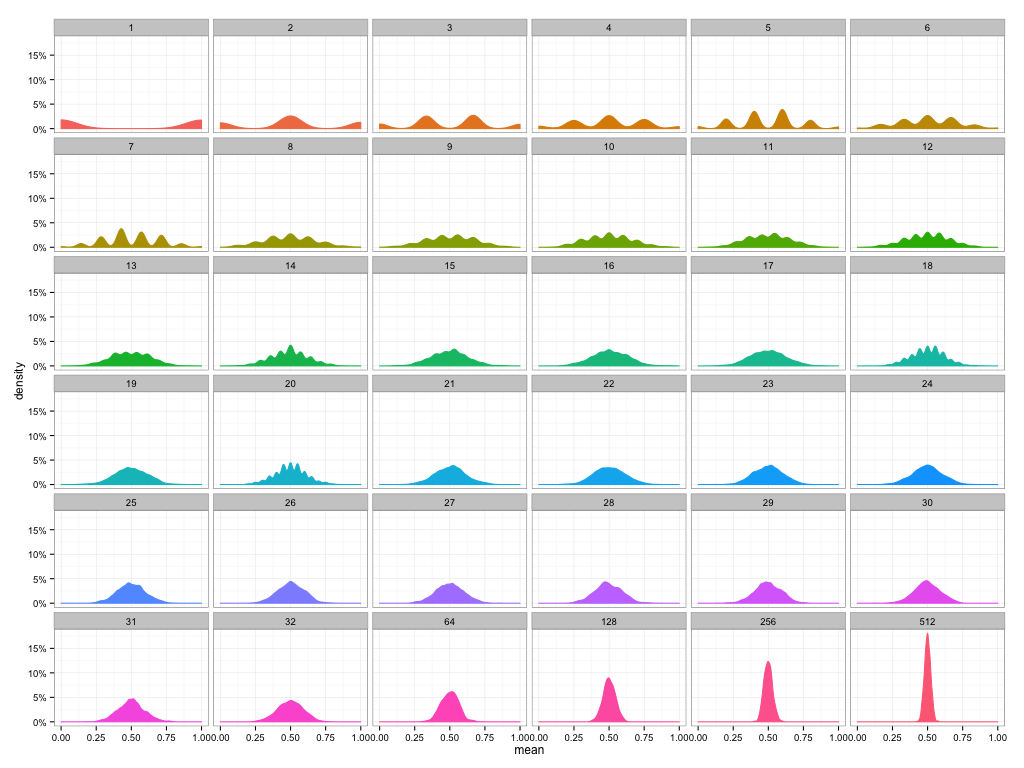
\includegraphics[width=0.8\linewidth]{clt.png}  
\caption{A Intuitive Example of Central Limit Theorem [I]} 
\label{fig1}
\end{figure}

\paragraph{Confidence Interval [3]}
Based on some sampling results, we may conclude with some level of certainty that a population parameter lies in some interval, and the interval is known as confidence interval.

In this section, we are particular interested in \textbf{lower bounded one-sided confidence interval} $[L,\infty)$, where with a $100(1-\alpha)\%$ lower confidence bound $L$ for population parameter $\theta$,
$$P[L\leq \theta] = 1-\alpha$$
\subsection{Mathematical Interpretation of $\bar{q}\geq (Q_n-\lambda s)$}
We need to satisfy the rule that the actual average quality of batch quantitative packaging of goods $\mu$ is greater or equal to the net quantity $Q_n$.

\subsubsection{Relations with Confidence Interval}
We are going to explain its relation to confidence interval from the interval estimation of mean $\overline{Q}$.

In terms of a sample following normal distribution, the value of $\sigma$ is unclear, thus needs to be estimated by $S$, the sample standard deviation. To find an one-sided $99.5\%$ confidence interval of the mean, we need the Student's T-Distribution:
$$T_{n-1} = \frac{\overline{Q}-\mu}{S/\sqrt{n}}$$

We use the similar notation defined in the slides [3]. Let $0<\alpha\leq 1$ we define $t_{\alpha,n}\geq 0$ by
$$\int^{\infty}_{t_{\alpha,n}} = \alpha/2$$

This can be visualized by the following figure.
\begin{figure}[!htbp] 
\centering 
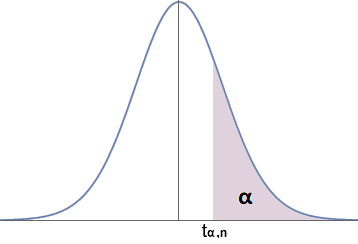
\includegraphics[width=0.6\linewidth]{t1l.png}  
\caption{Lower Bounded Integral Estimation of a Student's T-Distribution} 
\label{fig1}
\end{figure}

We now derive the one-sided confidence interval of the sample mean.\\

\fbox{
  \parbox{\textwidth}{
\paragraph{Theorem}
A $100(1-\alpha)\%$ upper confidence bound on $\mu$ is given by $\overline{Q}+\displaystyle\frac{st_{\alpha,n-1}}{\sqrt{n}}$.
  }
}

\newpage

The proof is simply as follows. From Student T-Distribution,
\begin{align*}
P[\frac{\overline{Q}-\mu}{S/\sqrt{n}}\geq -t_{\alpha,n-1}] &= 1-\alpha\\
P\big[\mu \leq \overline{Q}+\frac{s\cdot t_{\alpha,n-1}}{\sqrt{n}}\big] &= 1-\alpha
\end{align*}

We noticed a term $t_{\alpha}$ defined in the Table 4 in [1]. Through above discussion, we find out the meaning of this notation.

\paragraph{Notation}
\begin{equation}
t_{1-\alpha} = \frac{t_{\alpha,n-1}}{\sqrt{n}}
\end{equation}

Using notation (1), we now have:
$$P[\mu \leq \overline{Q}+ st_{\alpha}] = 1-\alpha$$
which indicates that for a batch of products with $\mu = Q_n$, 
\begin{align*}
P[Q_n \leq \overline{Q}+ st_{\alpha}] &= 1-\alpha\\
P[\overline{Q} \geq Q_n - st_{\alpha}] &= 1-\alpha
\end{align*}

We have $99.5\%$ confidence that the batch will be accepted, if the sample mean $\overline{q}$ satisfies that:
$$\overline{q} \geq Q_n - st_{\alpha}$$
 
For verification that our assumption is correct, we calculated the theoretic modifying factor $\lambda$ for given $n$ and compare with given $n$.

\begin{table}[!htbp]
  \centering
    \begin{tabular}{ccc}
    \hline
    Sample Size n & Theoretic $\lambda$ & Given $\lambda$ in Table 4 \\
    \hline
    10    & 1.027688233 & 1.028 \\
    13    & 0.847176855 & 0.848 \\
    50    & 0.379002443 & 0.379 \\
    80    & 0.295105589 & 0.295 \\
    125   & 0.233987509 & 0.234 \\
    \hline
    \end{tabular}%
   \caption{Theoretic and Given Modifying Factors}
\end{table}

We observed that the values correspond. 
\subsubsection{Relations with Hypothesis Test}
\paragraph{Relations with Neyman-Pearson Hypothesis Test}
In a Neyman-Pearson Null Hypothesis Test, we basically want to make a decision between two discrete hypothesis by accepting one of them.

To explain this table in the view of Neyman-Pearson Hypothesis Test, we set out the hypotheses as:
$$H_0: \mu = Q_n$$
$$H_1: |\mu-Q_n| \geq \delta$$
and try to choose between them.

To set up the test, we need to select a test statistic and define a critical region. From Section 3.4.1, with a probability of $1-\alpha$,
$$T_{n-1} \geq -t_{\alpha,n-1}$$

If $H_0$ is true,
$$P[\frac{\overline{Q}-Q_n}{S/\sqrt{n}}<-t_{-\alpha,n-1}] = \alpha$$
giving the critical region
$$\overline{q} < Q_n - \frac{st_{-\alpha,n-1}}{\sqrt{n}}$$

Therefore, the sample data with $\overline{q} \geq Q_n - \lambda = Q_n - \displaystyle\frac{st_{-\alpha,n-1}}{\sqrt{n}}$ falls out of the critical region, and we hence fail to reject $H_0$. 

Since $\alpha = 0.005$, the chance of this being an error is only $0.005$. Note that this implies that a lot is acceptable unless proven otherwise.

\paragraph{Relations with Fisher's Hypothesis Test}
In a Fisher's Null Hypothesis Test, we basically look for evidence against some hypothesis $H_0$. From [3], we know that the P Value (level of significance) is the upper bound of the probability obtaining the data when the hypothesis is true, i.e.
$$P=P[D\ |\ H_0]$$

To explain this table in the view of Fisher's Null Hypothesis Test, we set out the null hypothesis as:
$$H_0: \mu = Q_n$$
and try to find evidence against it.

In the following we will verify that the inequality $\bar{q}\geq (Q_n-\lambda s)$ ensures that a batch with $\mu=Q_n$ will be rejected at no more than 0.005 level of significance, as is required in [1, section 5.3.2.1].

We assume the same definition of $t_{\alpha}$ from Section 3.4.1. From definition, the P value can be calculated by the following one-sided interval:
\begin{align*}
P[D\ |\ H_0]
&= P[\overline{Q} \geq Q_n - t_{\alpha}s\ |\ \mu = Q_n]\\
&= P[\overline{Q} \geq \mu - t_{\alpha}s]\\
&= P[\overline{Q} \geq \mu - \frac{t_{\alpha,n-1}s}{n}]\\
&= P[\frac{\overline{Q}-\mu}{S/\sqrt{n}}\geq - t_{\alpha,n-1}]\\
&= 1-\alpha
\end{align*}

In [3, Table 4], it's preset that $\alpha = 0.995$. Hence the P value is given by $P = 0.005$, which is small enough to reject $H_0$.

Therefore, there is evidence that $\mu$ is greater than $Q_n$ if we received a sample data with $\overline{q}\geq Q_n-\lambda$.

\newpage

\subsection{Relations between Confidence Interval and Hypothesis Tests}
From the above discussion of the two-tailed null hypothesis
$$H_0: \mu = Q_n$$

We conclude that:
\begin{itemize}
\item Neyman-Pearson: \\
$\overline{q}$ lies in the critical region of $\alpha$ $\Leftrightarrow$ null value $Q_n$ does not lie in the $100(1-\alpha\%$ one-sided upper bounded confidence interval for $\mu$.
\item Fisher's: \\
$H_0$ will be rejected at $\alpha$ level of significance $\Leftrightarrow$ null value $Q_n$ does not lie in the $100(1-\alpha)\%$ one-sided upper bounded confidence interval for $\mu$.
\end{itemize}

\section{Acceptance Sampling for Net Quantities of a Batch}
\subsection{Objectives}
This section is oriented to question ii).

The objective of this section is to:
\begin{itemize}
\item calculate the significance of producer's and customer's risks;
\item verify the validity of the acceptance numbers $c$ that the document preset.
\end{itemize} 

After the section, readers should be able to comprehend:
\begin{itemize}
\item how risks are controlled through the significance level;
\item how the acceptance numbers were derived under the restrictions of producer's risk $\alpha$, customer's risk $\beta$ and type $T_2$ shortfall.
\end{itemize} 
In the process, readers will be shown a series of figures to visualize the concept.

\subsection{Definition and Notation}
\paragraph{Acceptance Sampling [3]}
In acceptance sampling, we apply the following notations:

We denote the batch number by $N$ and sample number by $n$ still. For the actual but unknown proportion of products with $T_1$ shortfall, we use the notation $\Pi$, and ideally we accept the batch if this proportion is less than $\Pi_0$. To lower the costumer's risk, we set another "barely acceptable" proportion $\Pi_1$.

Upon that, we make two one-sided hypotheses:
$$H_0: \Pi\leq \Pi_0$$
$$H_1: \Pi>\Pi_1$$

In sample testing, we define acceptance number $c$ that if the number of defectives is less than or equal to $c$, we accept the batch of products.

\paragraph{Ignorance of $T_2$ Shortfall}
In the fifth and sixth column, the testing method is similar to the precess of acceptance sampling, except that "defective items" are divided in to $T_1$ shortfall and $T_2$ shortfall.

\textbf{In the following section, we will approximate the test by the acceptance sampling process, by assuming that no $T_2$ shortfall happens. To validate this assumption, we will prove that $T_2$ shortfalls are ignorable when the $Q_n$ is large and $\sigma$ is small.}

From Central Limit Theorem, we assumed that the net quantity $Q$ of a unit product follows a normal distribution with variance $\mu$ and standard deviation $\sigma$. We further assume that $\mu\approx Q_n$.

The probability of detecting an $T_1$ shortfall is given by
\begin{align*}
P[Q_n-2T \leq Q < Q_n-T]
&= P[\frac{Q_n-2T-\mu}{\sigma} \leq \frac{Q-\mu}{\sigma} < \frac{Q_n-T-\mu}{\sigma}]\\
&= P[\frac{Q_n-2T-\mu}{\sigma} \leq Z < \frac{Q_n-T-\mu}{\sigma}]\\
&= \Phi(\frac{Q_n-T-\mu}{\sigma})-\Phi(\frac{Q_n-2T-\mu}{\sigma})\\
&= \Phi(\frac{-T}{\sigma})-\Phi(\frac{-2T}{\sigma})\\
\end{align*}

The probability of detecting an $T_2$ shortfall is given by
\begin{align*}
P[Q < Q_n-2T]
&= P[\frac{Q-\mu}{\sigma}<\frac{Q_n-2T-\mu}{\sigma}]\\
&= P[Z<\frac{Q_n-2T-\mu}{\sigma}]\\
&= \Phi(\frac{-2T}{\sigma})\\
\end{align*}

We denote the ratio $k:=\displaystyle\frac{P[Q < Q_n-2T]}{P[Q_n-2T \leq Q < Q_n-T]}$, which measures the probability of and $T_2$ shortfall compare to $T_1$. 

\newpage

Using \texttt{Mathematica}, we plot $k$ against $\sigma$ (ranging between 0 and 1) and $Q_n$ (ranging between 0 and 10). The plot is given by:

\begin{figure}[!htbp] 
\centering 
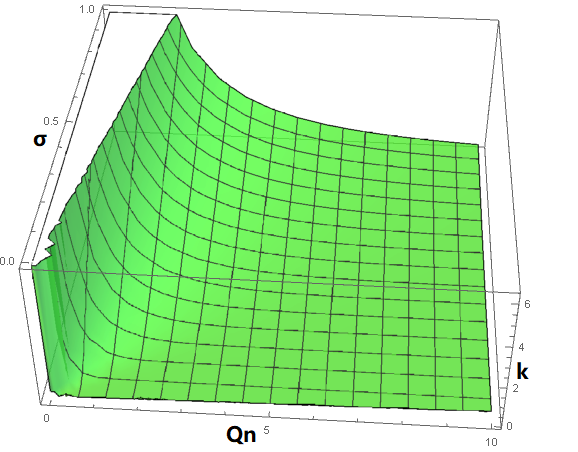
\includegraphics[width=0.6\linewidth]{T12.png}  
\caption{The Plot of $k$ against $\sigma$ and $Q_n$} 
\label{fig1}
\end{figure}

Reading from Figure 4 we directly note that $T_2$ shortfalls are ignorable when the $Q_n$ is large and $\sigma$ is small. For example, we fix $\sigma=0.4$ and $\mu=Q_n=8$, we can calculate the $k$ value is only:
$$k = 0.00444795$$

However, situations when the batch has a large $\sigma$ and small $Q_n$ will be discussed at the end of this section.

\subsection{Calculation of Significance Level}
\subsubsection{Level of Type I Error}
The significance Level of Type I Error is known as producer's risk $\alpha$, which highlights the probability of rejecting an acceptable batch by mistake. From definition,
\begin{align*}
\alpha
&= P[\text{reject }H_0\ |\ H_0 \text{ is true}]\\
&= P[d\geq c\ |\ \Pi\leq \Pi_0]\\
&\leq P[d\geq c\ |\ \Pi = \Pi_0]\\
&= \sum_{d\geq c} \displaystyle\frac{\tbinom{r}{d}\tbinom{N-r}{n-d}}{\tbinom{N}{n}}
\end{align*}

In [1, Section 5.3.2.2], the document preset that in the acceptance sampling,
$$\Pi_0 = 0.0025$$
which we can apply in the above formula and find the value of $\alpha$.

\paragraph{Hypergeometeric Distribution}
From above discussion, we have derived a formula:
$$\alpha = \sum_{d\geq c} \displaystyle\frac{\tbinom{r}{d}\tbinom{N-r}{n-d}}{\tbinom{N}{n}}$$
where $c$ is a function of $n$, $n$ is a function of $N$, and
$$r = N\Pi = N\Pi_0$$

Hence, we derive a function of $\alpha$ against $N$:
\begin{equation}
\alpha(N) = \sum_{d\geq c} \displaystyle\frac{\tbinom{N\Pi_0}{d}\tbinom{N(1-\Pi_0)}{n(N)-d}}{\tbinom{N}{n(N)}}
\end{equation}

Using \texttt{Matlab}, we can plot the function as follows.
\begin{figure}[!htbp] 
\centering 
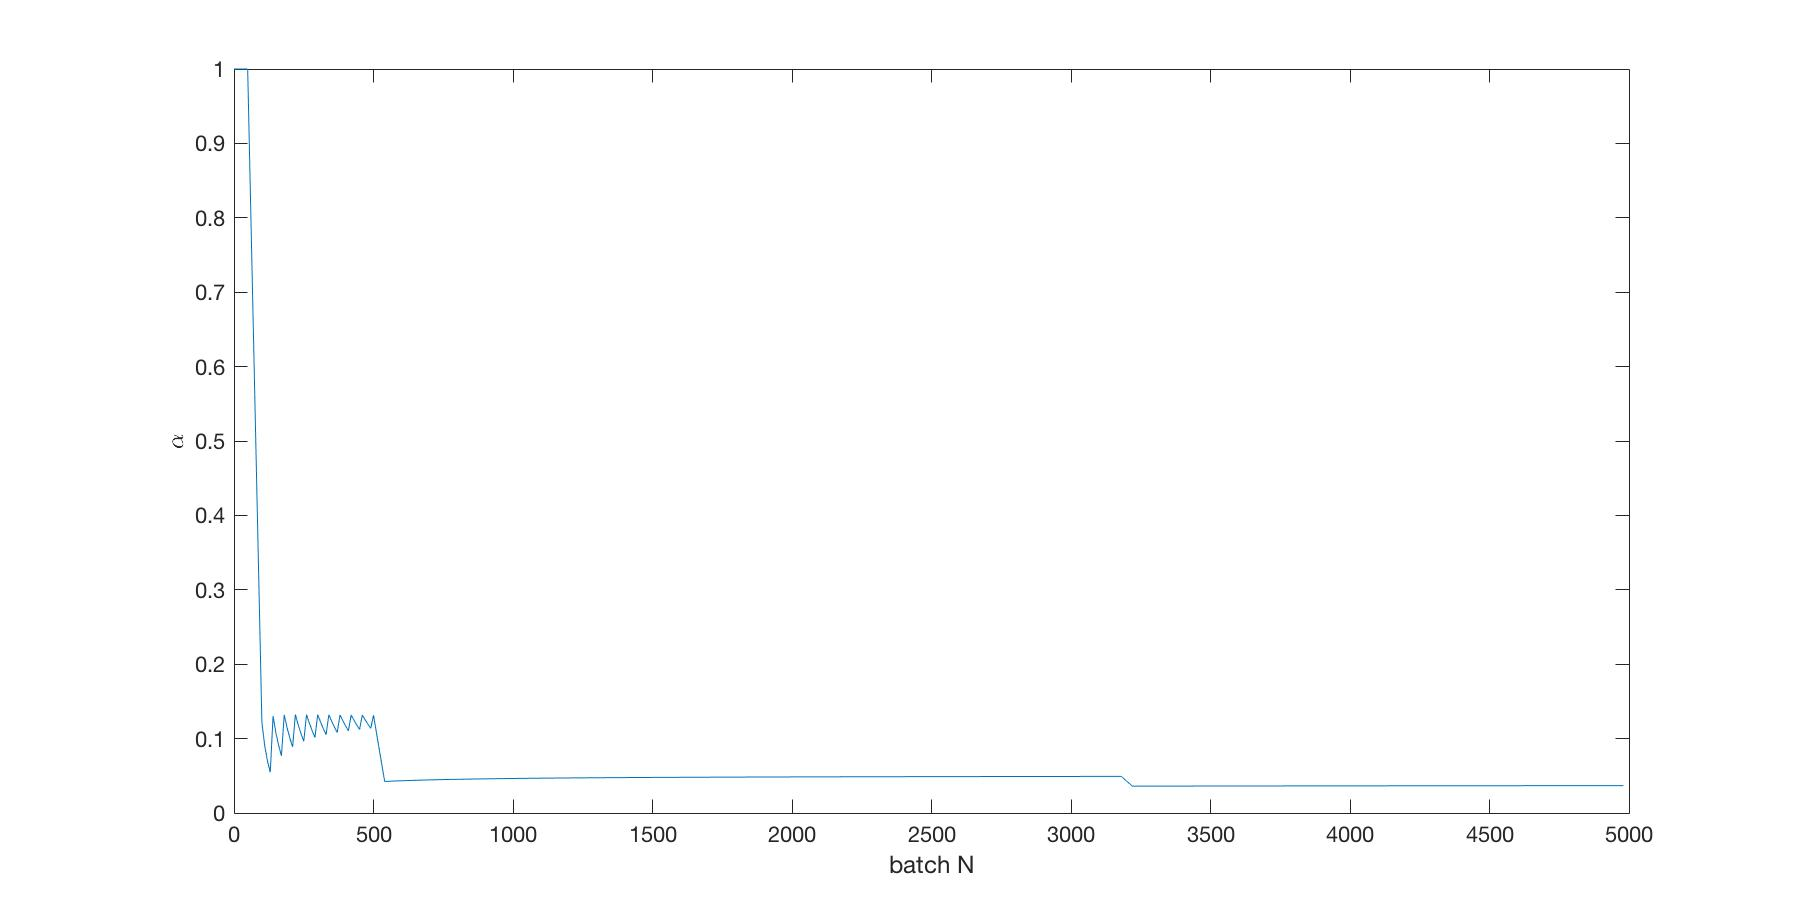
\includegraphics[width=1\linewidth]{alpha-N.jpg}  
\caption{The Relationship between $\alpha$ and $N$} 
\end{figure}

\paragraph{Binomial Distribution}
We can use a Binomial Distribution as approximation to eliminate large $N$ in
$$\alpha = \sum_{d\geq c} \displaystyle\frac{\tbinom{r}{d}\tbinom{N-r}{n-d}}{\tbinom{N}{n}}$$

By $p = \displaystyle\frac{r}{N}=\Pi=\Pi_0$, we have
$$\alpha \approx \sum_{d\geq c}\tbinom{n}{d}\Pi_0^d(1-\Pi_0)^{n-d}$$

Plugging in the given data, we found
\begin{table}[!htbp]
  \centering
    \begin{tabular}{|c|c|c|c|c|c|}
    \hline
    n     & 10    & 13    & 50    & 80    & 125 \\
    \hline
    c     & 0     & 1     & 3     & 5     & 7 \\
    \hline
    $\alpha$ (binomial) & 1     & 0.28045161 & 0.12937796 & 0.05036913 & 0.03815242 \\
    \hline
    \end{tabular}%
    \caption{$\alpha$ with Corresponding $n$ in Binomial Approx}
\end{table}%

\paragraph{Poisson Distribution}
We can use a Poisson Distribution as approximation to eliminate large $N$ in
$$\alpha = \sum_{d\geq c} \displaystyle\frac{\tbinom{r}{d}\tbinom{N-r}{n-d}}{\tbinom{N}{n}}$$

By $k = \displaystyle\frac{nr}{N}=n\Pi=n\Pi_0$, we have
$$\alpha \approx \sum_{d\geq c} \frac{(n\Pi_0)^de^{-\Pi_0}}{d!}$$

Plugging in the given data, we found
\begin{table}[!htbp]
  \centering
    \begin{tabular}{|c|c|c|c|c|c|}
    \hline
    n     & 10    & 13    & 50    & 80    & 125 \\
    \hline
    c     & 0     & 1     & 3     & 5     & 7 \\
    \hline
    $\alpha$ (poisson) & 1     & 0.27747265 & 0.13153233 & 0.05265302 & 0.04020872 \\
    \hline
    \end{tabular}%
    \caption{$\alpha$ with Corresponding $n$ in Poisson Approx}
\end{table}%

We found the value of $\alpha$ unacceptably large for small $n$. This will be discussed in Section 6, question iv).
\subsubsection{Level of Type II Error}
The significance Level of Type II Error is known as customer's risk $\alpha$, which highlights the probability of accepting an unacceptable batch by mistake. From definition,
\begin{align*}
\beta
&= P[\text{failing to reject }H_0\ |\ H_1 \text{ is true}]\\
&= P[d\leq c\ |\ \Pi > \Pi_1]\\
&= \sum_{d\leq c} \displaystyle\frac{\tbinom{r}{d}\tbinom{N-r}{n-d}}{\tbinom{N}{n}}\\
&= \sum_{d\leq c} \displaystyle\frac{\tbinom{n\Pi}{d}\tbinom{(1-\Pi)N}{n-d}}{\tbinom{N}{n}}
\end{align*}

We know that $\beta(\Pi)$ is a function of $\Pi$, and it is meaningless to analyse $N$ in $\beta$ when $\Pi$ is unknown, therefore, we apply approximations.

\paragraph{Binomial Distribution}
We can use a Binomial Distribution as approximation to eliminate large $N$ by $p = \displaystyle\frac{r}{N}=\Pi=\Pi_0$:

$$\beta \approx \sum_{d\leq c}\tbinom{n}{d}\Pi^d(1-\Pi)^{n-d}$$

Using \texttt{Matlab}, we can plot the function $\beta$ v.s. $\Pi$:

\begin{figure}[!htbp] 
\centering 
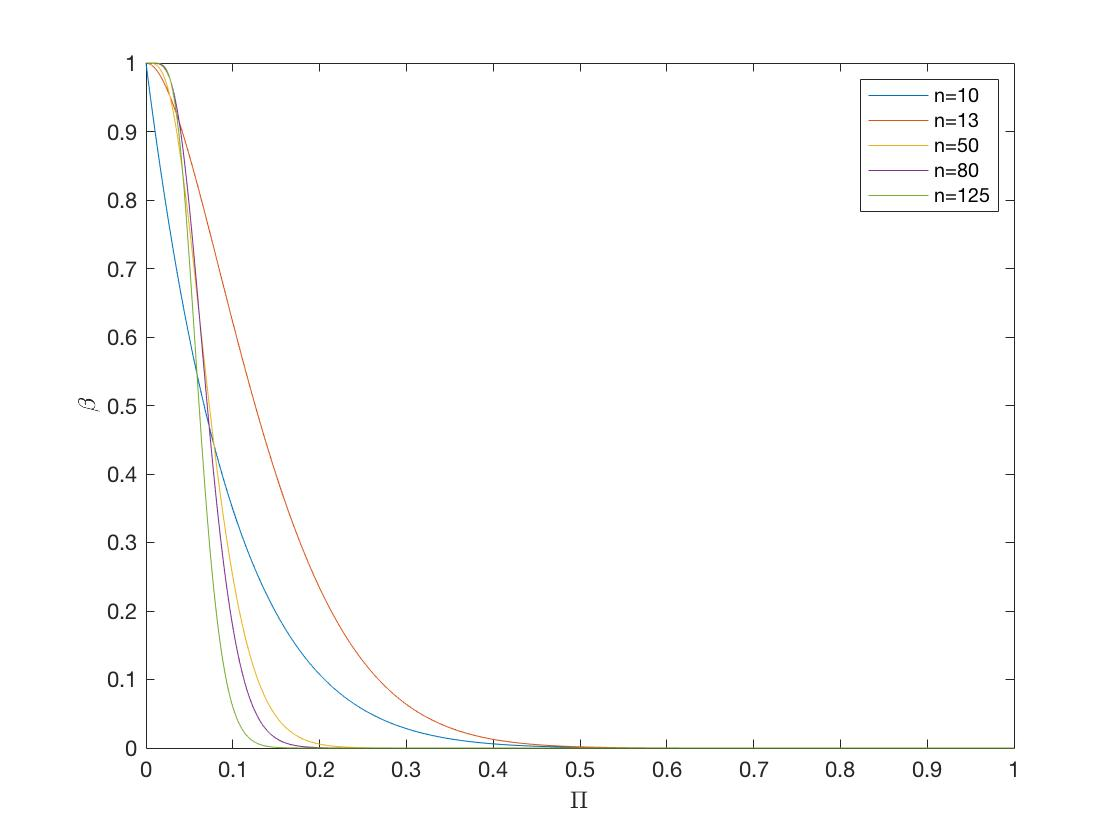
\includegraphics[width=0.6\linewidth]{beta-pi-b.jpg}  
\caption{The Relationship between $\beta$ and $\Pi$, Binomial Approx} 
\end{figure}

\paragraph{Poisson Distribution}
We can use a Poisson Distribution as approximation to eliminate large $N$ by $k = \displaystyle\frac{nr}{N}=n\Pi=n\Pi_0$:

$$\beta \approx \sum_{d\leq c} \frac{(n\Pi)^de^{-\Pi}}{d!}$$

Using \texttt{Matlab}, we can plot the function $\beta$ v.s. $\Pi$:

\begin{figure}[!htbp] 
\centering 
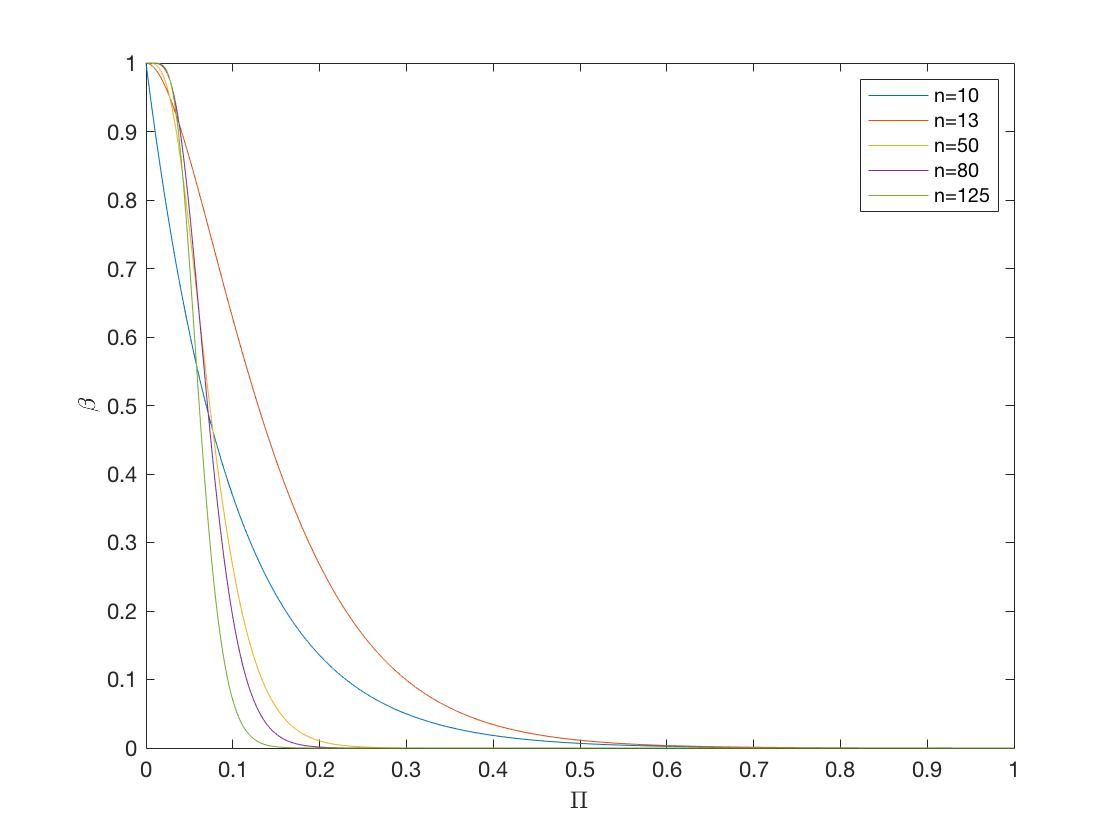
\includegraphics[width=0.6\linewidth]{beta-pi-p.jpg}  
\caption{The Relationship between $\beta$ and $\Pi$, Poisson Approx} 
\end{figure}

In [1, Section 5.3.3], the document preset that in the acceptance sampling, we want to verify the value of $\beta$ when
$$\Pi = 0.09$$

Given the value of $\Pi$, we can now calculate the value of $\beta$ for each $n$ using Poisson and Binomial Distribution Approximation, and plot the function of $\beta$ against $N$ for the original Hypergeometric formula, by plugging $\Pi=0.09$ in the previously derived formulae:

Hypergeometeric:
$$\beta =  \sum_{d\leq c} \displaystyle\frac{\tbinom{n\Pi}{d}\tbinom{(1-\Pi)N}{n-d}}{\tbinom{N}{n}}$$

Binomial:
$$\beta \approx \sum_{d\leq c}\tbinom{n}{d}\Pi^d(1-\Pi)^{n-d}$$

Poisson:
$$\beta \approx \sum_{d\leq c} \frac{(n\Pi)^de^{-\Pi}}{d!}$$

The results are as follows.

\begin{table}[!htbp]
  \centering
    \begin{tabular}{|c|c|c|c|c|c|}
    \hline
    n     & 10    & 13    & 50    & 80    & 125 \\
    \hline
    c     & 0     & 1     & 3     & 5     & 7 \\
    \hline
    $\beta$ (poisson) & 0.78  & 0.96  & 0.96  & 0.98  & 0.99  \\
    \hline
    $\beta$ (binomial) & 0.78  & 0.96  & 0.96  & 0.98  & 0.99  \\
    \hline
    \end{tabular}%
    \caption{The value of $\beta$ found for $\Pi=9\%$.}
\end{table}%

\begin{figure}[!htbp] 
\centering 
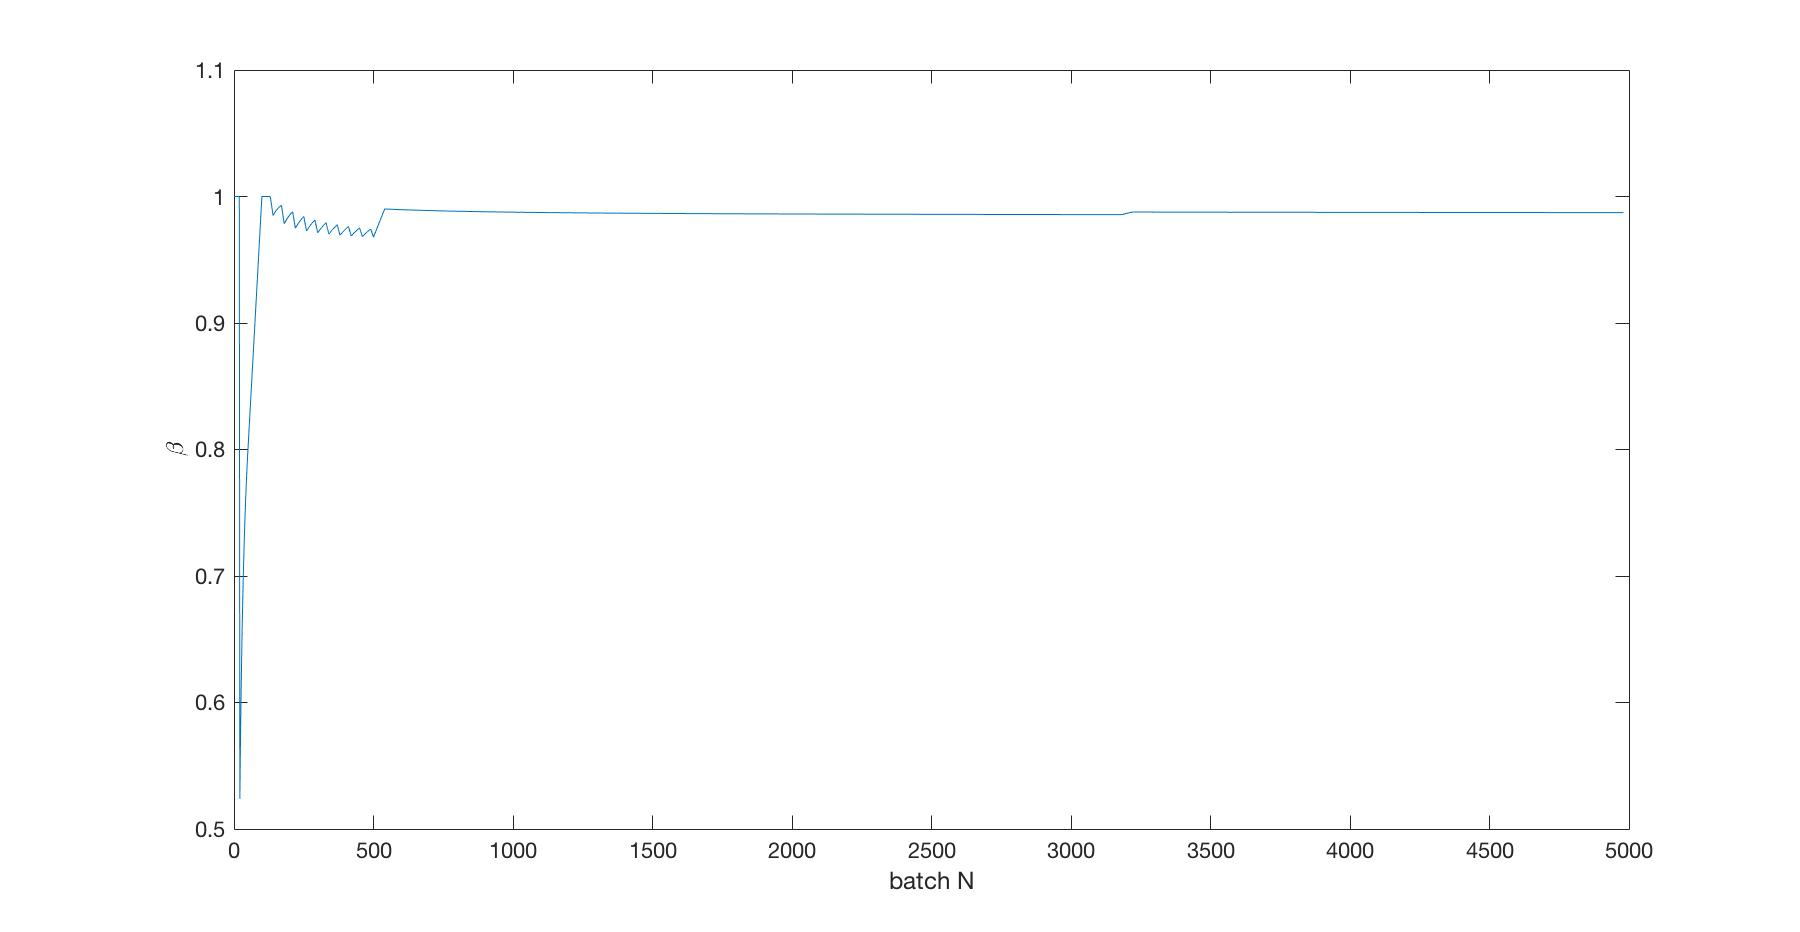
\includegraphics[width=1\linewidth]{beta-N.jpg}  
\caption{The Relationship between $\beta$ and $N$, Hypergeometric, at $\Pi=0.09$.} 
\end{figure}

\newpage

\subsection{Derivation of Acceptable Number}
In this subsection, we first try to find the minimum and maximum of the acceptance number $c$, and shoot some deviations we found. Then, we apply a new method using OC Curves to find the adequate $c$, and give illustrative examples.

\subsubsection{Significance of $\alpha$ Determining $c_{\min}$}
In [1, Section 5.3.2.2], the document preset that in the acceptance sampling,
$$\Pi_0 = 0.0025$$
$$\alpha \leq 0.05$$

Plugging these parameters into the equalities that we derived in Section 4.3.1, we can find out the minimum integer number $c$ as the acceptance number.

In the following paragraphs, we basically want to plot a function of $c_{\min}$ versus $N$, and read out the $c$ from the plot.

\paragraph{Hypergeometric Distribution}
The original value of $\alpha$ is found from Hypergeometric distribution:
$$\alpha = \sum_{d\geq c} \displaystyle\frac{\tbinom{r}{d}\tbinom{N-r}{n-d}}{\tbinom{N}{n}}\leq 0.05$$

We want to find the function of $c_{\min}$ v.s. $N$, but the function is complicated and in fact it takes \texttt{Matlab} a few minutes for calculations. Mathematically, we limited the parameters:
\begin{enumerate}
\item The value of $d$.

To make sure that the codes run well, we set restrictions that:
$$\max(0,n-N+r)\leq d \leq \min(n,r)$$
\item The value of $r$.

The number $r$ should be integer. For accuracy, we set:
$$r = \text{round}(N\Pi_0)$$

\item The value of $c$ should be integer.
\end{enumerate}

\newpage

The plot is given as:
\begin{figure}[!htbp] 
\centering 
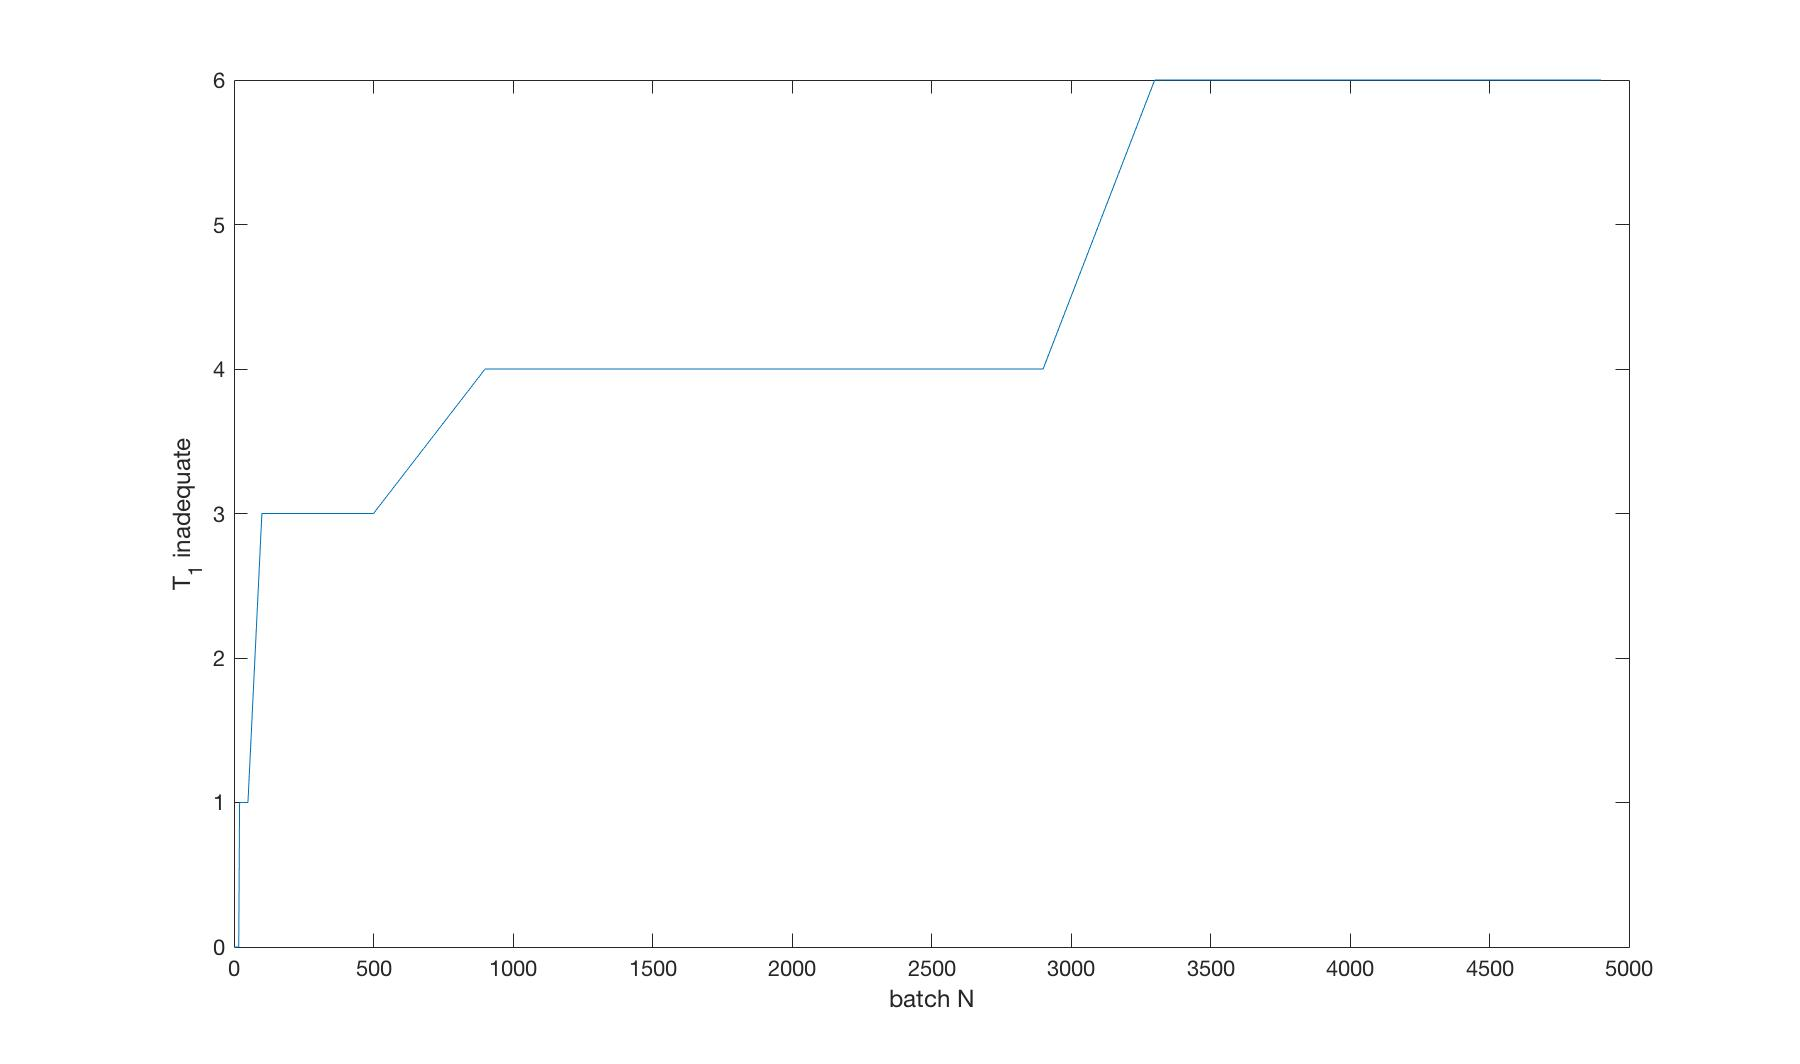
\includegraphics[width=1\linewidth]{alpha-hyper.jpg}  
\caption{The Relationship between $c_{\min}$ and $N$, Hypergeometeric} 
\end{figure}

From the plot, we read out that:
\begin{table}[!htbp]
  \centering
    \begin{tabular}{ccc}
    \hline
    Sample Size n & Given Acceptance Number $c$ & Theoretic $c_{\min}$ from Hypergeometeric \\
    \hline
    10    & 0     & 0 \\
    13    & 1     & 1 \\
    50    & 3     & 3 \\
    80    & \cellcolor[rgb]{ .851,  .882,  .949}5 & \cellcolor[rgb]{ .851,  .882,  .949}4 \\
    125   & \cellcolor[rgb]{ .851,  .882,  .949}7 & \cellcolor[rgb]{ .851,  .882,  .949}6 \\
    \hline
    \end{tabular}%
    \caption{$c_{\min}$ given by Hypergeometric}
\end{table}%

We observed a good correspondence for smaller $N$, as all the $c_{\min}$ are smaller than the given $c$.

\newpage

\paragraph{Binomial Distribution}
We also have the Binomial approximated $\alpha$:
$$\alpha \approx \sum_{d\geq c}\tbinom{n}{d}\Pi_0^d(1-\Pi_0)^{n-d}$$
which gives good approximations for larger $N$.

Doing the same thing, we obtained the following Figure from \texttt{Matlab}.
\begin{figure}[!htbp] 
\centering 
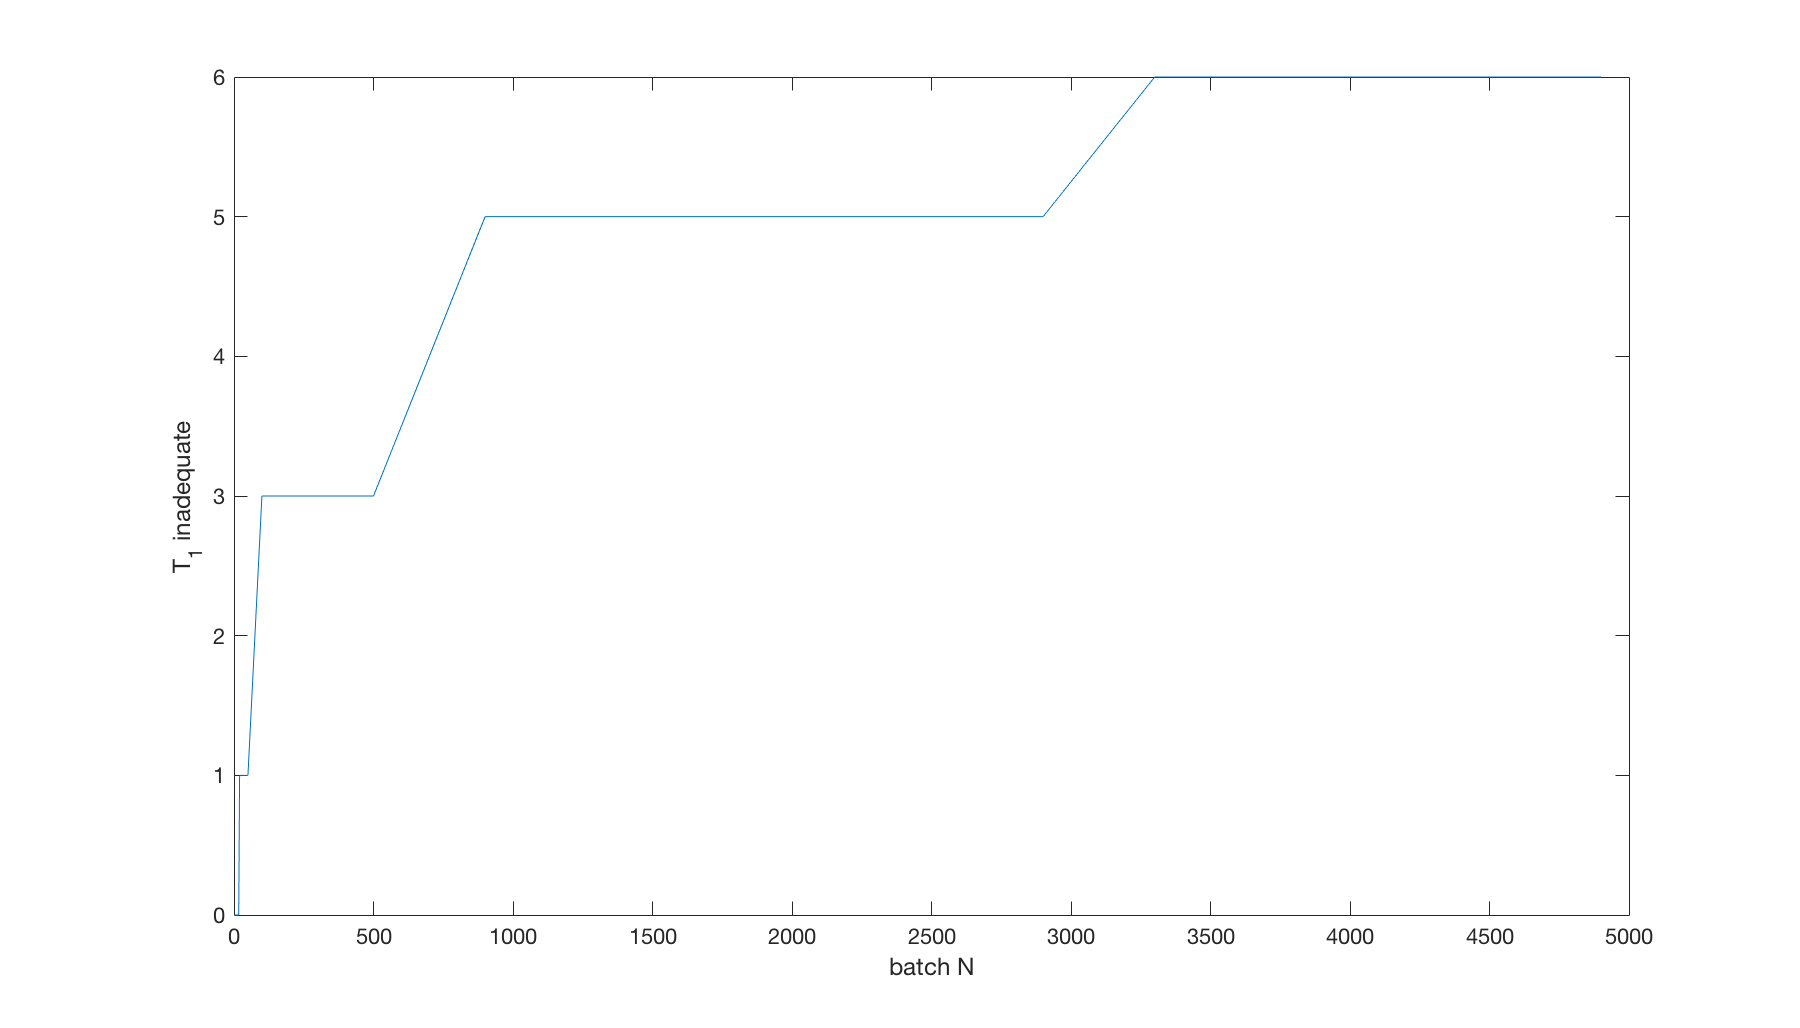
\includegraphics[width=1\linewidth]{alpha-bino.png}  
\caption{The Relationship between $c_{\min}$ and $N$, Binomial Approx} 
\end{figure}

From the plot, we read out that:
\begin{table}[!htbp]
  \centering
    \begin{tabular}{ccc}
    \hline
    Sample Size n & Given Acceptance Number $c$ & Theoretic $c_{\min}$ from Binomial \\
    \hline
    10    & 0     & 0 \\
    13    & 1     & 1 \\
    50    & 3     & 3 \\
    80    & 5     & 5 \\
    125   & \cellcolor[rgb]{ .851,  .882,  .949}7 & \cellcolor[rgb]{ .851,  .882,  .949}6 \\
    \hline
    \end{tabular}%
    \caption{$c_{\min}$ given by Binomial}
\end{table}%

We observed a better correspondence for smaller $N$, as all the $c_{\min}$ are smaller than the given $c$, and for $n=80$, the calculated $c$ coincide with given ones.

\newpage

\paragraph{Poisson Distribution}
We also have the Poisson approximated $\alpha$:
$$\alpha \approx \sum_{d\geq c} \frac{(n\Pi_0)^de^{-\Pi_0}}{d!}$$
which gives good approximations for larger $N$.

Doing the same thing, we obtained the following Figure from \texttt{Matlab}.
\begin{figure}[!htbp] 
\centering 
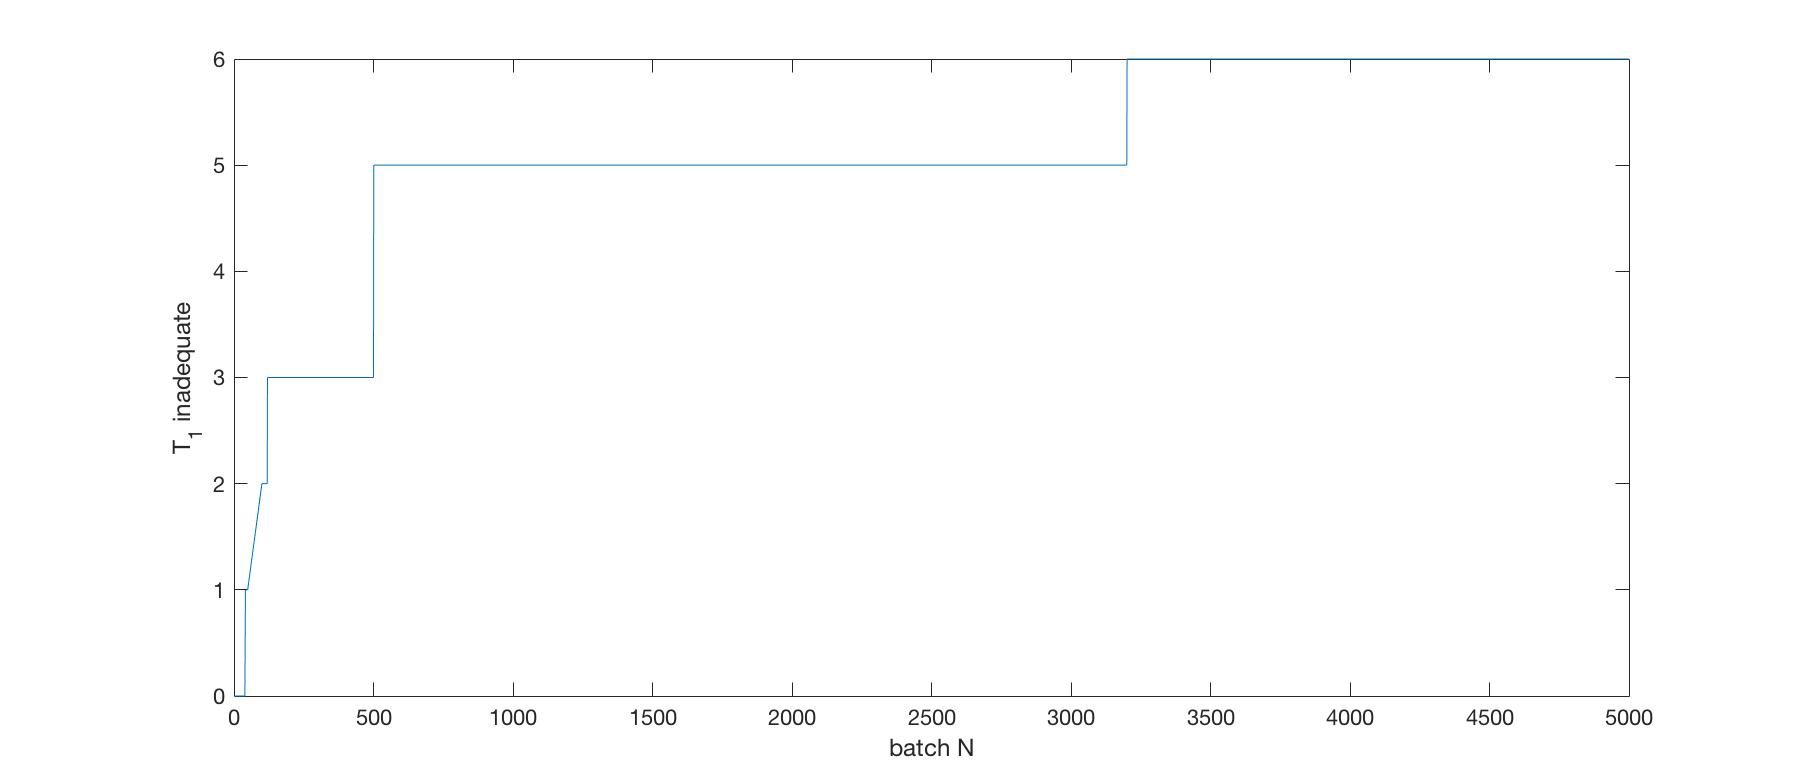
\includegraphics[width=1\linewidth]{alpha-pois.jpg}  
\caption{The Relationship between $c_{\min}$ and $N$, Poisson Approx} 
\end{figure}

From the plot, we read out that:
\begin{table}[!htbp]
  \centering
    \begin{tabular}{ccc}
    \hline
    Sample Size n & Given Acceptance Number$c$ & Theoretic $c_{\min}$ from Poisson \\
    \hline
    10    & 0     & 0 \\
    13    & 1     & 1 \\
    50    & \cellcolor[rgb]{ .851,  .882,  .949}3     & \cellcolor[rgb]{ .851,  .882,  .949}2,3 \\
    80    & 5     & 5 \\
    125   & \cellcolor[rgb]{ .851,  .882,  .949}7 & \cellcolor[rgb]{ .851,  .882,  .949}6 \\
    \hline
    \end{tabular}%
    \caption{$c_{\min}$ given by Poisson}
\end{table}%

We observed a good correspondence for smaller $N$, as all the $c_{\min}$ are smaller than the given $c$, but not as good as Binomial.

\newpage

\subsubsection{Significance of $\beta$ Determining $c_{\max}$}
In [1, Section 5.3.3], the document preset that in the acceptance sampling,
$$\Pi = 0.09$$
$$1 - \beta \geq 0.9 \Rightarrow \beta \leq 0.1$$

Plugging these parameters into the equalities that we derived in Section 4.3.1, we can find out the maximum integer number $c$ as the acceptance number.

In the following paragraphs, we basically want to plot a function of $c_{\max}$ versus $N$, and read out the $c$ from the plot.

\paragraph{Hypergeometric Distribution}
The original value of $\alpha$ is found from Hypergeometric distribution:
$$\beta = \sum_{d\leq c} \displaystyle\frac{\tbinom{n\Pi}{d}\tbinom{(1-\Pi)N}{n-d}}{\tbinom{N}{n}} \leq 0.1$$

We want to find the function of $c_{\max}$ v.s. $N$, similarly, the plot is given as:
\begin{figure}[!htbp] 
\centering 
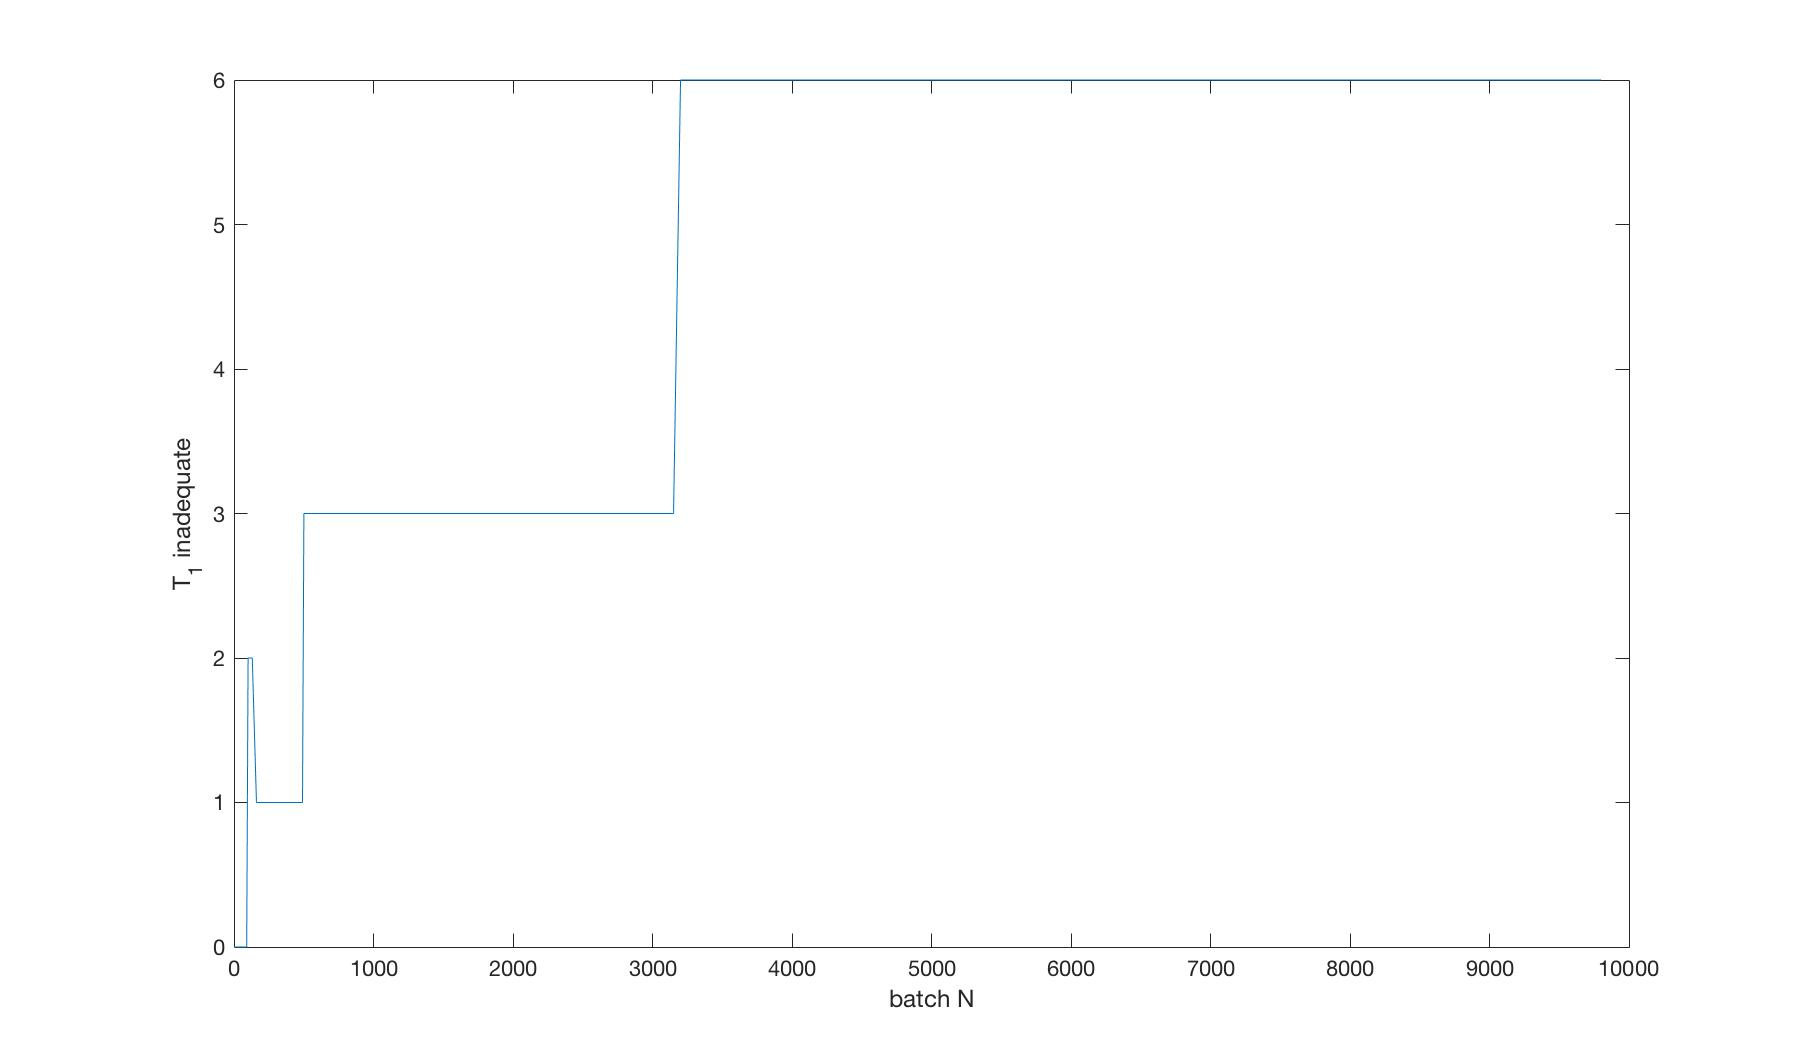
\includegraphics[width=1\linewidth]{beta-hyper.jpg}  
\caption{The Relationship between $c_{\max}$ and $N$, Hypergeometeric} 
\end{figure}

\newpage

From the plot, we read out that:
\begin{table}[!htbp]
  \centering
    \begin{tabular}{ccc}
    \hline
    Sample Size n & Given Acceptance Number $c$ & Theoretic $c_{\min}$ from Hypergeometeric \\
    \hline
    10    & 0     & 0 \\
    13    & \cellcolor[rgb]{ .851,  .882,  .949}1     & \cellcolor[rgb]{ .851,  .882,  .949}1,2 \\
    50    & \cellcolor[rgb]{ .851,  .882,  .949}3     & \cellcolor[rgb]{ .851,  .882,  .949}1 \\
    80    & \cellcolor[rgb]{ .851,  .882,  .949}5     & \cellcolor[rgb]{ .851,  .882,  .949}3 \\
    125   & \cellcolor[rgb]{ .851,  .882,  .949}7     & \cellcolor[rgb]{ .851,  .882,  .949}6 \\
    \hline
    \end{tabular}%
    \caption{$c_{\max}$ given by Hypergeometric}
\end{table}%

The correspondence for larger $N$ is bad, because the maximum $c$ calculated turned out to be less than the given $c$.

\paragraph{Binomial Distribution}
Similarly, we repeat the process with Binomial approximation:
$$\beta \approx \sum_{d\leq c}\tbinom{n}{d}\Pi^d(1-\Pi)^{n-d}$$

The plot is given by
\begin{figure}[!htbp] 
\centering 
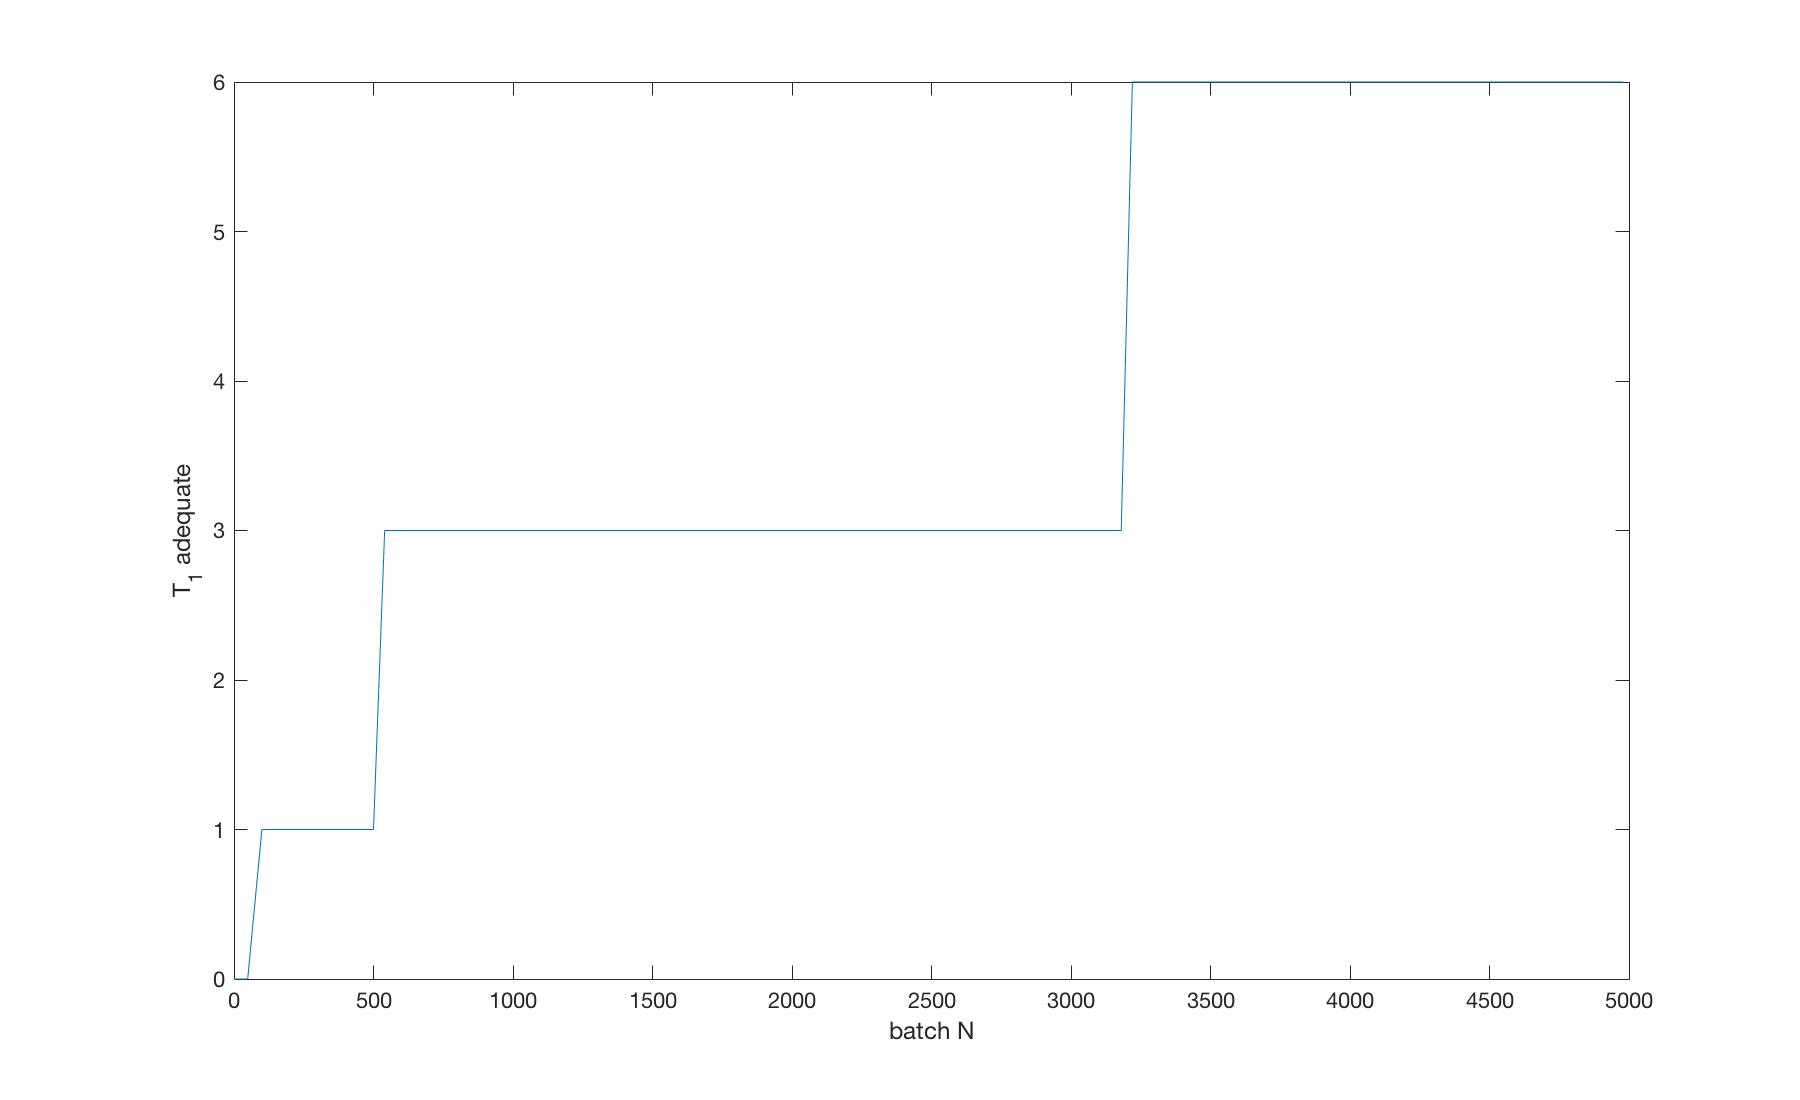
\includegraphics[width=1\linewidth]{beta-bino.jpg}  
\caption{The Relationship between $c_{\max}$ and $N$, Binomial} 
\end{figure}

\newpage

From the plot, we read out that:
\begin{table}[!htbp]
  \centering
    \begin{tabular}{ccc}
    \hline
    Sample Size n & Given Acceptance Number $c$ & Theoretic $c_{\min}$ from Binomial \\
    \hline
    10    & 0     & 0 \\
    13    & 1     & 1 \\
    50    & \cellcolor[rgb]{ .851,  .882,  .949}3     & \cellcolor[rgb]{ .851,  .882,  .949}1 \\
    80    & \cellcolor[rgb]{ .851,  .882,  .949}5     & \cellcolor[rgb]{ .851,  .882,  .949}3 \\
    125   & \cellcolor[rgb]{ .851,  .882,  .949}7     & \cellcolor[rgb]{ .851,  .882,  .949}6 \\
    \hline
    \end{tabular}%
    \caption{$c_{\max}$ given by Binomial}
\end{table}%

The correspondence for larger $N$ is still bad, because the maximum $c$ calculated turned out to be less than the given $c$.

\paragraph{Poisson Distribution}
$$\beta \approx \sum_{d\leq c} \frac{(n\Pi)^de^{-\Pi}}{d!}$$

The plot is given by
\begin{figure}[!htbp] 
\centering 
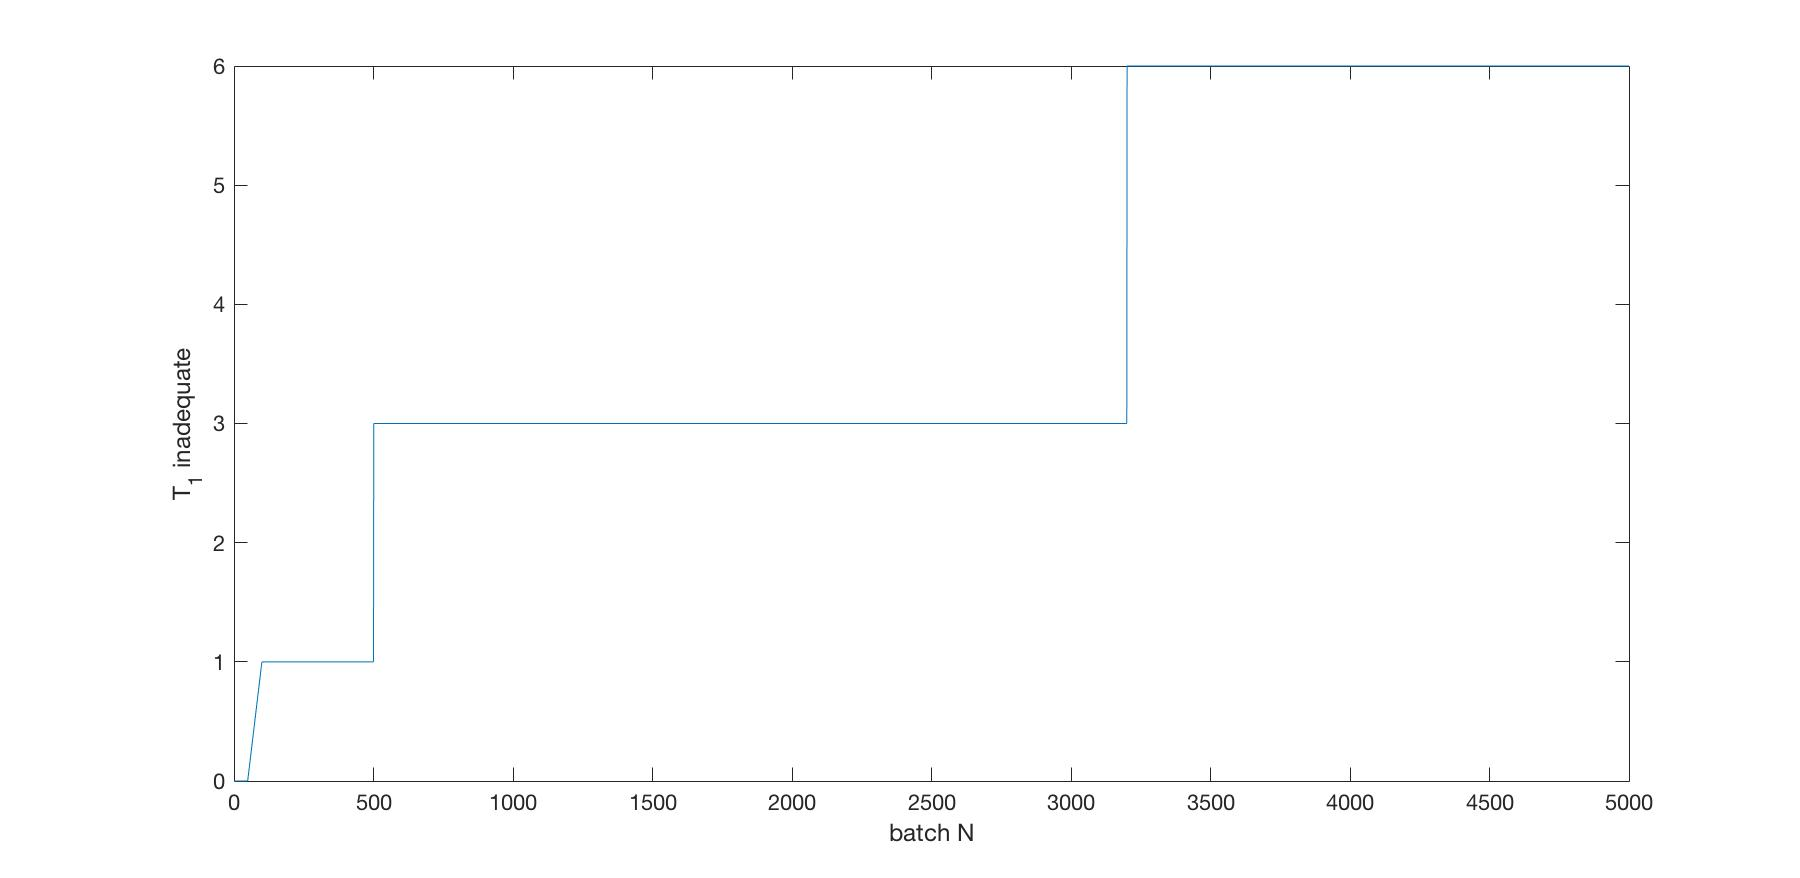
\includegraphics[width=1\linewidth]{beta-pois.jpg}  
\caption{The Relationship between $c_{\max}$ and $N$, Poisson} 
\end{figure}

\newpage

From the plot, we read out that:
\begin{table}[!htbp]
  \centering
    \begin{tabular}{ccc}
    \hline
    Sample Size n & Given Acceptance Number $c$ & Theoretic $c_{\min}$ from Poisson \\
    \hline
    10    & 0     & 0 \\
    13    & 1     & 1 \\
    50    & \cellcolor[rgb]{ .851,  .882,  .949}3     & \cellcolor[rgb]{ .851,  .882,  .949}1 \\
    80    & \cellcolor[rgb]{ .851,  .882,  .949}5     & \cellcolor[rgb]{ .851,  .882,  .949}3 \\
    125   & \cellcolor[rgb]{ .851,  .882,  .949}7     & \cellcolor[rgb]{ .851,  .882,  .949}6 \\
    \hline
    \end{tabular}%
    \caption{$c_{\max}$ given by Poisson}
\end{table}%

The correspondence for larger $N$ is still bad, because the maximum $c$ calculated turned out to be less than the given $c$.

We found that $\alpha$ gives almost perfect lower bound of $c$, but $beta$ fails to correspond to $c$ for the larger $N$. To look into this problem, we apply OC Curves for analysis.
\subsubsection{Determine $c$ from OC Curves}
In the previous examples, we basically fix the value of $\Pi$ and look for the relationship of bounds of $c$ with $N$. We found that for $n \geq 50$, the results are not corresponding. Now, we would like to fix the value of $n$, and plot the OC Curves with abscissa $\Pi$ by approximations.

The formula for the OC Curves is given by
\begin{align*}
P[\text{accpet }H_0]
&= P[d\leq c]\\
&= \sum_{d\leq c} \displaystyle\frac{\tbinom{N\Pi}{d}\tbinom{N(1-\Pi)}{n-d}}{\tbinom{N}{n}}\\
&\approx \sum_{d\leq c} \frac{(n\Pi)^de^{-\Pi}}{d!} \qquad (\text{Poisson Approx})
\end{align*}

We apply Poisson approximation since $n\geq 50$ is large enough, and we can plot the OC Curves with testing parameter $c$. Since $\alpha$ and $\beta$ require that
$$\Pi_0=0.025, \qquad \alpha\leq 0.05$$
$$\Pi=0.09, \qquad \beta\leq 0.1$$

On the OC Curves, we make auxiliary lines for $\alpha$:
$$P = 1-\alpha = 0.995$$
$$\Pi = \Pi_0 = 0.025$$
and for $\beta$:
$$P = \beta = 0.1$$
$$\Pi = 0.09$$

The OC Curves for each given $n$ are plotted as follows by \texttt{Matlab}.

\newpage

\begin{figure}[!htbp] 
\centering 
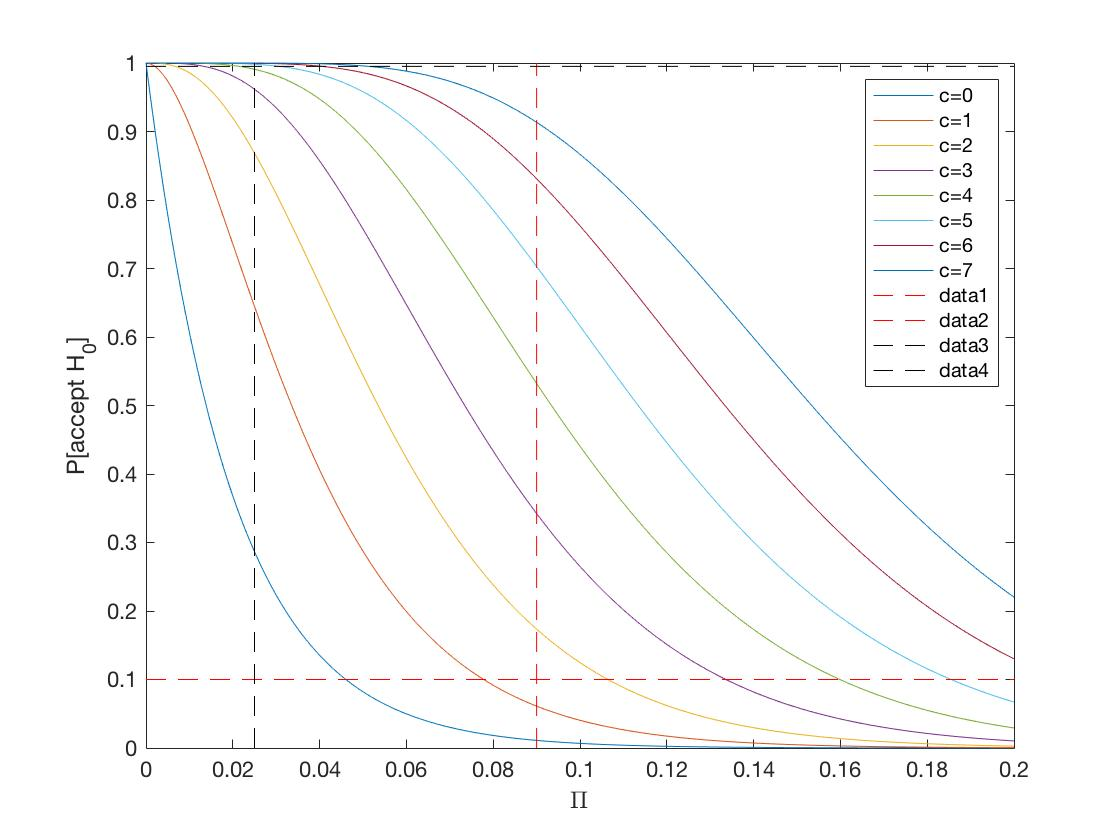
\includegraphics[width=0.7\linewidth]{n=50.jpg}  
\caption{OC Curves when $n = 50$} 
\end{figure}

For $n=50$, we read from the plot that $\alpha$ requires $c>4$ and $\beta$ requires $c<2$. Clearly it's not possible so we seek for middle solution. We found that the customer's risk is unreasonably high for larger $c$, and the producer's risk gets larger for smaller $c$. Therefore, we choose a middle solution $c=3$.

\begin{figure}[!htbp] 
\centering 
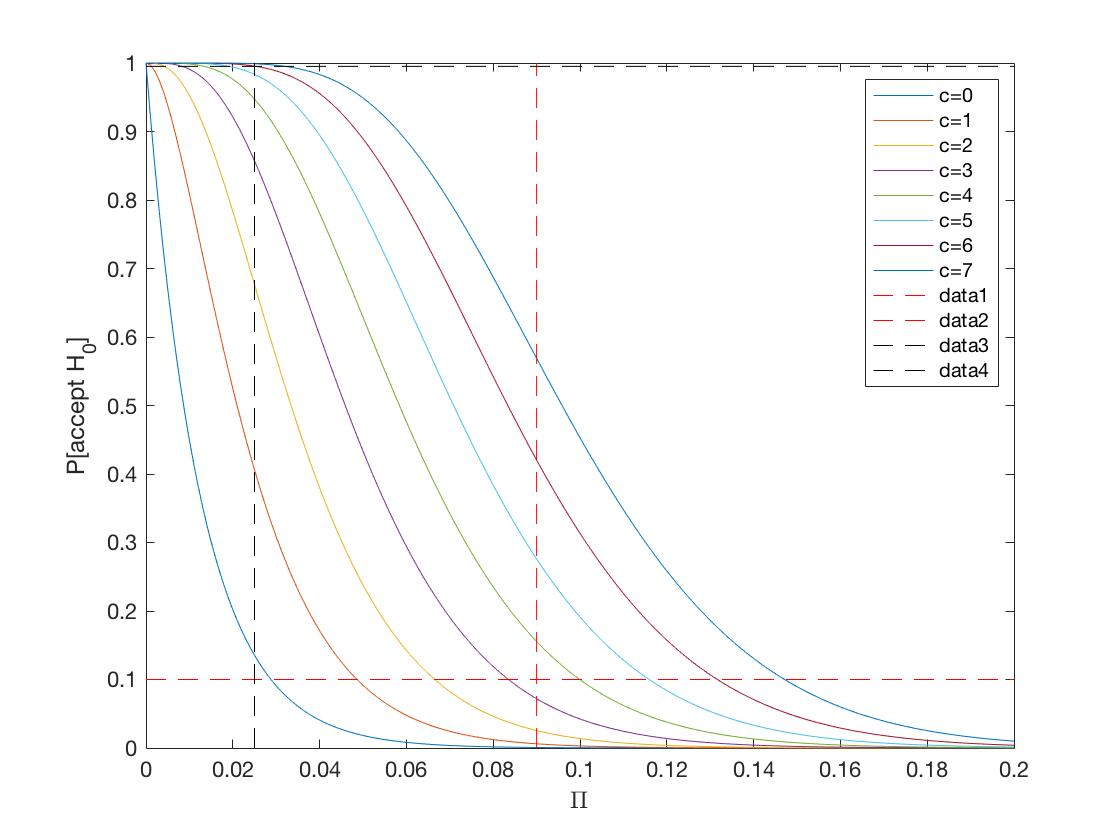
\includegraphics[width=0.7\linewidth]{n=80.jpg}  
\caption{OC Curves when $n = 80$} 
\end{figure}

For $n=80$, we read from the plot that $\alpha$ requires $c>5$ and $\beta$ requires $c<4$. Clearly it's not possible so we seek for middle solution. We found that the customer's risk is unreasonably high for larger $c$, and the producer's risk gets larger for smaller $c$. Therefore, we choose a middle solution $c=5$.

\newpage

\begin{figure}[!htbp] 
\centering 
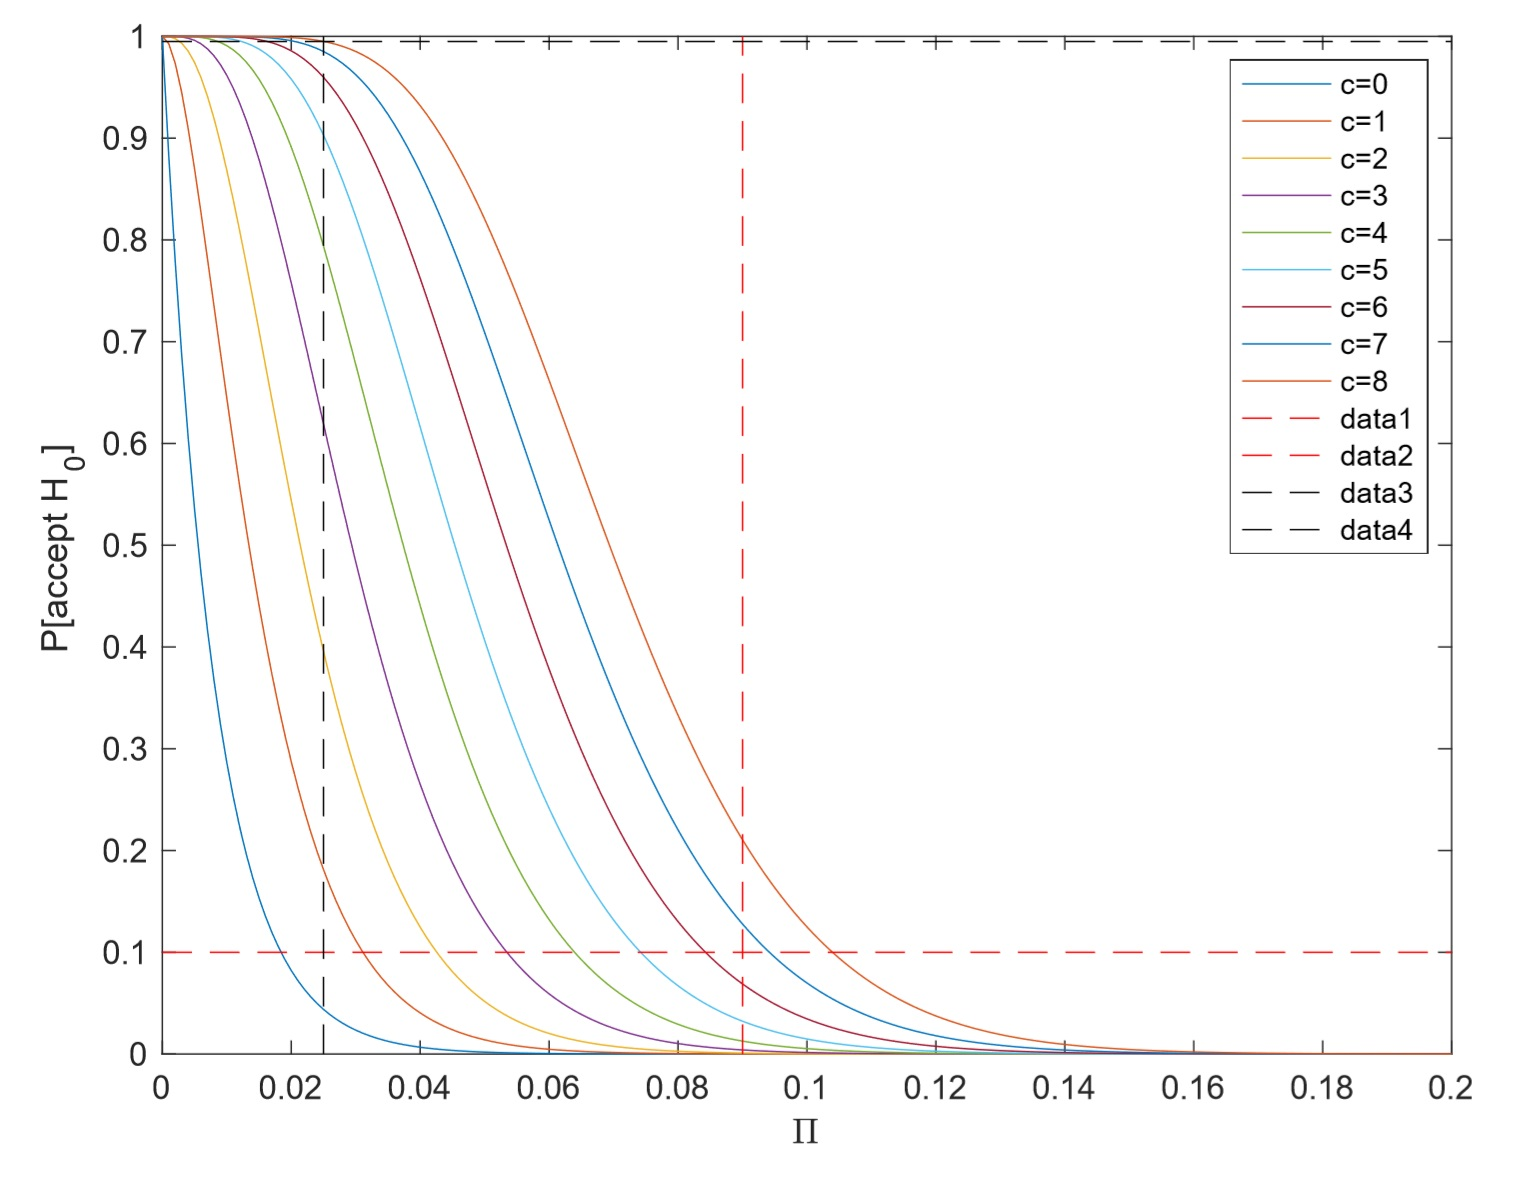
\includegraphics[width=0.8\linewidth]{n=125.jpg}  
\caption{OC Curves when $n = 125$} 
\end{figure}

For $n=125$, we read from the plot that $\alpha$ requires $c>7$ and $\beta$ requires $c<7$. Clearly it's not possible so we seek for middle solution. We found that the customer's risk is unreasonably high for larger $c$, and the producer's risk gets larger for smaller $c$. Therefore, we choose a middle solution $c=7$.

However, there is still some deviations from what we expected. Detailed discussion and modelling we be included in Section 6, oriented to question iv).
\section{Non-central T Distribution}
\subsection{Objectives}
The objective of this section is to look into the non-central T distribution where $T$-test involves. In this section, we will discuss some properties of this distribution, and applied it to the derivation of OC Curves and shortfall probability.

\subsection{Definition and Notations}
\paragraph{Operating Characteristic Curve (OC Curve)[3]}
With the help of OC Curves, people can evaluate non-normal distributions, where finding the integral is impractical.

In a hypothesis test with null hypothesis $H_0$, a single \textit{OC Curve} is a plot of $P[\text{accepting }H_0]$, the probability of accepting(failing to reject) $H_0$, versus $\theta$, some population parameter. The single curves each correspond a particular choice of test parameters.

\paragraph{$T$-Test[3]}
Let $X_1,\cdots,X_n$ be a random sample of size $n$ from a normal distribution with sample mean $\overline{X}$ and sample variance $S^2$. The normal distribution has unknown standard deviation $\sigma$, unknown population mean $\mu$ and we set up $\mu_0$ as a null value of $\mu$, and denote the difference 
$$\delta := \mu-\mu_0.$$

In our discussion, the OC Curves for T-Test feature an abscissa $d$ defined by
$$d := \frac{\mu-\mu_0}{\sigma}=\frac{\delta}{\sigma}$$

\paragraph{Non-central T-Distribution[4]} 
The \textit{non-central T-Distribution} is a generalization of \textit{Student's T-Distribution}, by adding a non-centrality parameter $\nu$. The following definition is based on [4], retrieved from \texttt{Wikipedia}.

Let $Z$ and $V_\gamma$ be independent random variables, where $Z$ follows \textit{Standard Normal Distribution} and $V_\gamma$ follows \textit{Chi-Squared Distribution}, with $\gamma$ degrees of freedom. Given $\nu\neq 0\in\mathbb{R}$, the random variable:
$$T_{\gamma,\nu} = \frac{Z+\nu}{\sqrt{V_\gamma/\gamma}}$$
is said to follow a Non-central T-Distribution with $\gamma$ degrees of freedom and non-centrality parameter $\nu$.

The direct formula of probability density function(PDF) and cumulative distribution function(CDF) of $T_{\gamma,\nu}$ are complicated and beyond discussion. Hence for short, we denote the PDF and CDF of $T_{\gamma,\nu}$ by $f_{\gamma,\nu}$ and $F_{\gamma,\nu}$.
\subsection{Derivation of the OC Curve}
\fbox{
  \parbox{\textwidth}{
\paragraph{Theorem}
The random variable
$$T_{n-1} = \frac{\overline{X}-\mu_0}{S/\sqrt{n}}$$
follows a non-central T-distribution with $n-1$ degrees of freedom and non-centrality parameter $d\sqrt{n}$.
  }
}

Inspired by Theorem 2.3.9 in [3], we basically want to construct a standard normal random variable and a chi-squared random variable in $T_{n-1}= \displaystyle\frac{\overline{X}-\mu_0}{S/\sqrt{n}}$.

The proof of this theorem is as follows. 
\begin{align*}
T_{n-1}
&= \frac{\overline{X}-\mu_0}{S/\sqrt{n}} \\
&= \frac{(\overline{X}-\mu)+(\mu-\mu_0)}{S/\sqrt{n}} \\
&= \frac{(\overline{X}-\mu)+\delta}{S/\sqrt{n}} \\
&= \frac{\displaystyle\frac{(\overline{X}-\mu)+\delta}{\sigma/\sqrt{n}}}{\displaystyle\frac{S/\sqrt{n}}{\sigma/\sqrt{n}}} \\
&= \frac{\displaystyle\frac{\overline{X}-\mu}{\sigma/\sqrt{n}}+\displaystyle\frac{\delta}{\sigma/\sqrt{n}}}{\sqrt{[(n-1)S^2/\sigma^2]/(n-1)}} \\
&= \frac{Z+\nu}{\sqrt{\chi^2_{n-1}/(n-1)}} \\
\end{align*}

We know that $Z = \displaystyle\frac{\overline{X}-\mu}{\sigma/\sqrt{n}}$ follows a standard normal distribution, and $\chi^2_{n-1} = \displaystyle\frac{(n-1)S^2}{\sigma^2}$ follows a chi-squared distribution with $n-1$ degrees of freedom.

Hence as is defined in Section 4.3, we conclude that $T_{n-1}$ is a non-central T distribution with $n-1$ degrees of freedom and the non-centrality parameter is given by
\begin{align*}
\nu 
&= \frac{\delta}{\sigma/\sqrt{n}}\\
&= \frac{\bcancel{\sigma}\cdot d}{\bcancel{\sigma}/\sqrt{n}}\\
&= d \sqrt{n}
\end{align*}

The proof is done.

The formula of the OC Curves is in essence a function of $P[\text{accepting }H_0]$ versus $\{d,\alpha,n\}$. In the $T$-Test, the null hypotheses $H_0$ can be either:
$$H_0:\ \mu = \mu_0$$
$$H_0:\ \mu \geq \mu_0$$
$$H_0:\ \mu \leq \mu_0$$

The following will discuss them one-by-one.

\paragraph{Derivation of OC Curve When $H_0:\ \mu = \mu_0$}
When we set
$$H_0:\ \mu = \mu_0,$$
we fix the critical region by $|t|>t_{\alpha/2,n-1}$ and reject $H_0$ at significance level $\alpha$ if
$$|T_{n-1}|>t_{\alpha/2,n-1}$$

We can then estimate the probability:
\begin{align*}
P[\text{accepting }H_0]
&= P[|T_{n-1}| \leq t_{\alpha/2,n-1}]\\
&= P[-t_{\alpha/2,n-1} \leq T_{n-1} \leq t_{\alpha/2,n-1}]\\
\end{align*}

As is proved in the previous theorem, $T_{n-1} = \displaystyle\frac{\overline{X}-\mu_0}{S/\sqrt{n}}$ follows non-central T-distribution with $n-1$ degrees of freedom and non-centrality parameter $d\sqrt{n}$. Hence we can represent the probability through integral estimation:

\begin{figure}[!htbp] 
\centering 
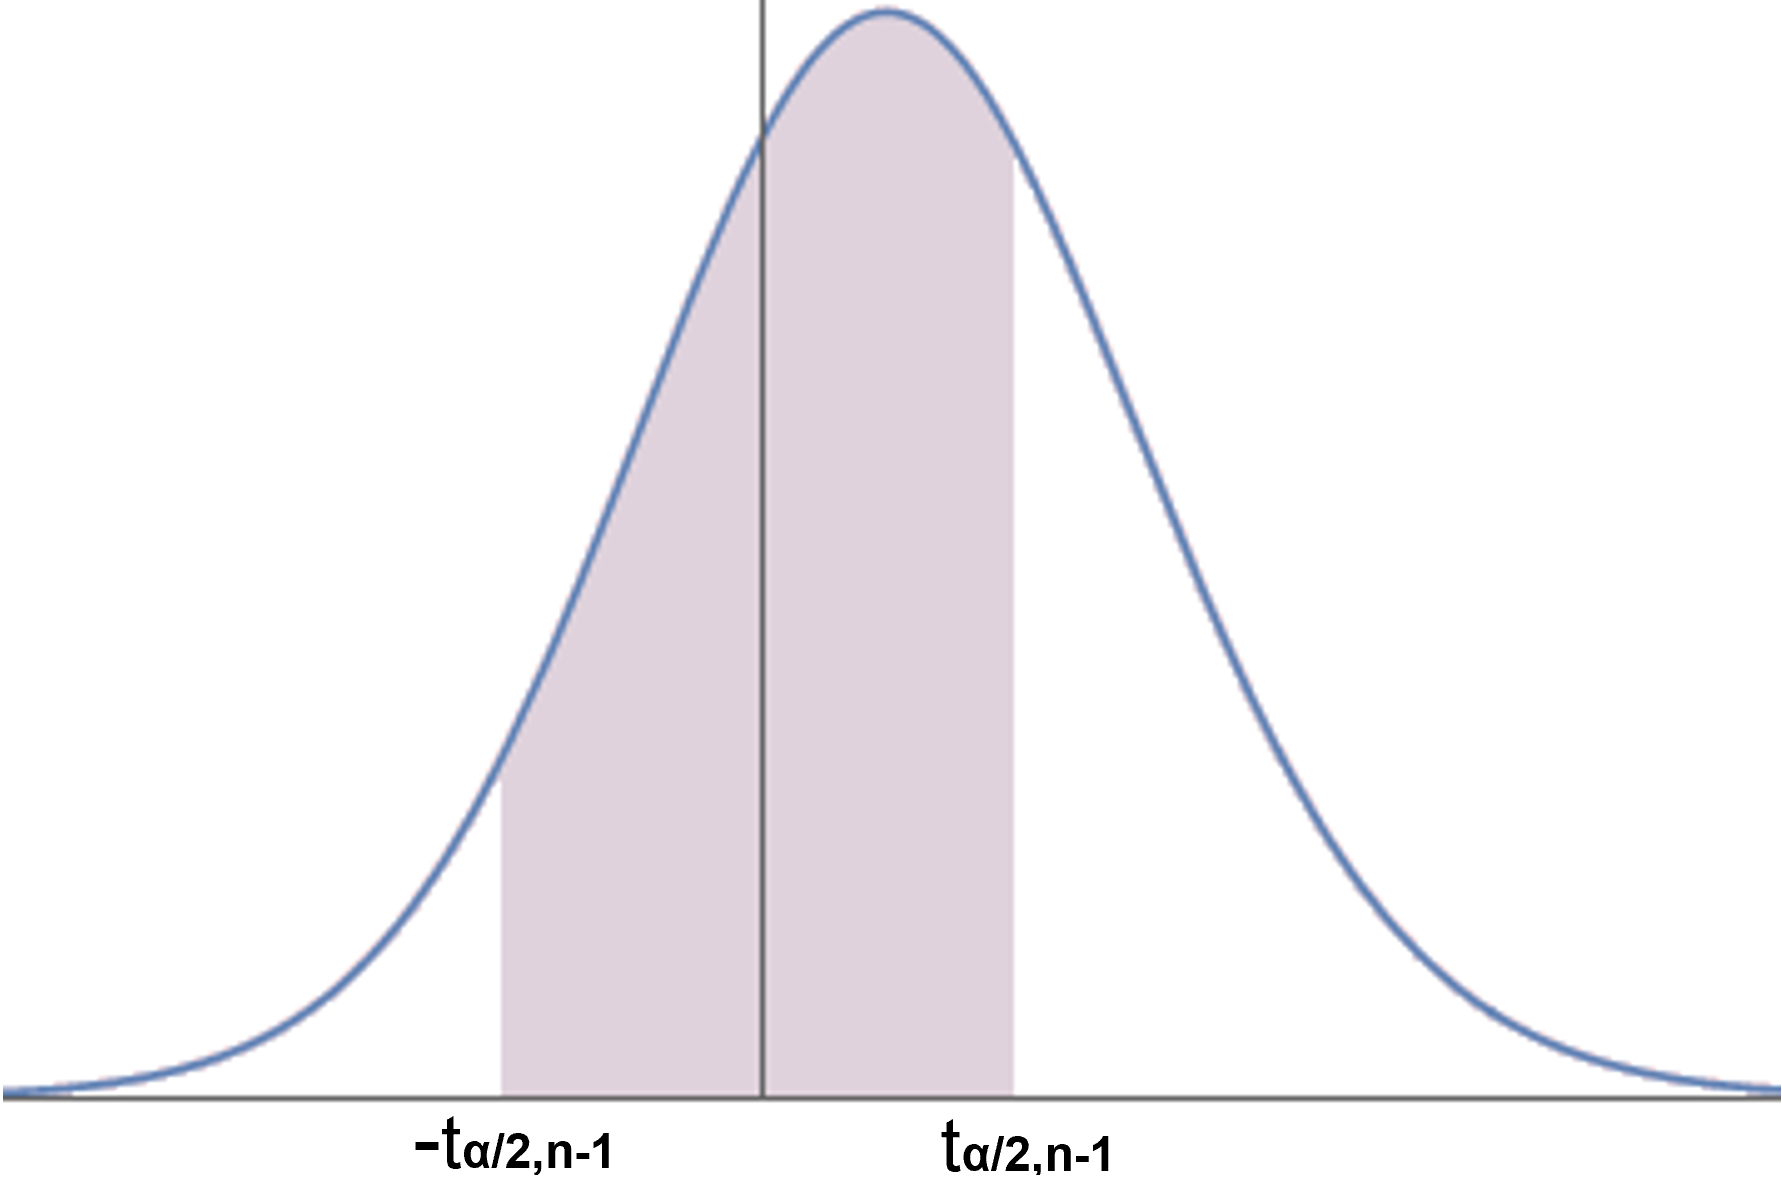
\includegraphics[width=0.6\linewidth]{nct2.png}  
\caption{Two-sided Integral Estimation of a Non-Central T-Distribution} 
\label{fig1}
\end{figure}

The probability is represented by the shadowed area and can be calculated by integral.
\begin{align*}
P[\text{accepting }H_0]
&= P[-t_{\alpha/2,n-1} \leq T_{n-1} \leq t_{\alpha/2,n-1}]\\
&= \int_{-t_{\alpha/2,n-1}}^{t_{\alpha/2,n-1}} f_{n-1,d\sqrt{n}}(x) dx\\
&= F_{n-1,d\sqrt{n}}(x)\big|_{-t_{\alpha/2,n-1}}^{t_{\alpha/2,n-1}}\\
&= F_{n-1,d\sqrt{n}}(t_{\alpha/2,n-1}) - F_{n-1,d\sqrt{n}}(-t_{\alpha/2,n-1})\\
\end{align*}

Through the above process, we successfully derived a formula for the OC Curve of the T-test in terms of the cumulative distribution function of the non-central T distribution for $H_0: \mu=\mu_0$:

$$P[\text{accepting }H_0]= F_{n-1,d\sqrt{n}}(t_{\alpha/2,n-1}) - F_{n-1,d\sqrt{n}}(-t_{\alpha/2,n-1})$$

\paragraph{Derivation of OC Curve When $H_0:\ \mu \leq \mu_0$}
When we set
$$H_0:\ \mu \leq \mu_0,$$
we fix the critical region by $t>t_{\alpha/2,n-1}$ and reject $H_0$ at significance level $\alpha$ if
$$T_{n-1}>t_{\alpha/2,n-1}$$

Again, we can then estimate the probability
$$P[\text{accepting }H_0] = P[T_{n-1} \leq t_{\alpha/2,n-1}]$$ through integral estimation:

\begin{figure}[!htbp] 
\centering 
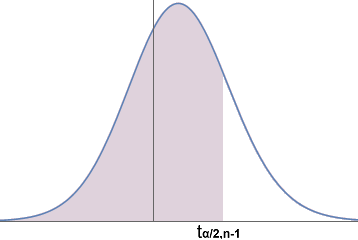
\includegraphics[width=0.6\linewidth]{nct1u.png}  
\caption{Upper Bounded One-sided Integral Estimation of a Non-Central T-Distribution} 
\end{figure}

The probability is represented by the shadowed area and can be calculated by integral.
\begin{align*}
P[\text{accepting }H_0]
&= P[T_{n-1} \leq t_{\alpha/2,n-1}]\\
&= \int_{-\infty}^{t_{\alpha/2,n-1}} f_{n-1,d\sqrt{n}}(x) dx\\
&= F_{n-1,d\sqrt{n}}(t_{\alpha/2,n-1})
\end{align*}

Hence the formula for the OC Curve of the T-test in terms of the cumulative distribution function of the non-central T distribution for $H_0: \mu\leq\mu_0$:

$$P[\text{accepting }H_0]= F_{n-1,d\sqrt{n}}(t_{\alpha/2,n-1})$$

\paragraph{Derivation of OC Curve When $H_0:\ \mu \geq \mu_0$}
When we set
$$H_0:\ \mu \geq \mu_0,$$
we fix the critical region by $t<t_{\alpha/2,n-1}$ and reject $H_0$ at significance level $\alpha$ if
$$T_{n-1}<t_{\alpha/2,n-1}$$

Again, we can then estimate the probability
$$P[\text{accepting }H_0] = P[T_{n-1} \geq t_{\alpha/2,n-1}]$$ through integral estimation:

\begin{figure}[!htbp] 
\centering 
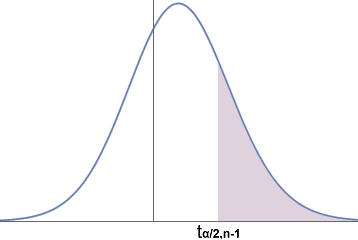
\includegraphics[width=0.6\linewidth]{nct1l.png}  
\caption{Lower Bounded One-sided Integral Estimation of a Non-Central T-Distribution} 
\end{figure}

The probability is represented by the shadowed area and can be calculated by integral.
\begin{align*}
P[\text{accepting }H_0]
&= P[T_{n-1} \geq t_{\alpha/2,n-1}]\\
&= \int_{t_{\alpha/2,n-1}}^{\infty} f_{n-1,d\sqrt{n}}(x) dx\\
&= 1-F_{n-1,d\sqrt{n}}(t_{\alpha/2,n-1})
\end{align*}

Hence the formula for the OC Curve of the T-test in terms of the cumulative distribution function of the non-central T distribution for $H_0: \mu\geq\mu_0$:

$$P[\text{accepting }H_0]= 1-F_{n-1,d\sqrt{n}}(t_{\alpha/2,n-1})$$
\subsection{The OC Curves of the Test in Table 4}
We can see from Part 4.3.2 that data from Table 4 fit the third condition in T-test, with null hypothesis
$$H_0: \mu=Q_n$$

The vertical coordinates of OC curve is P[accepting $H_0$] and it is related to $n, d, \alpha$. n and $\alpha$ are testing variables and d is $\displaystyle\frac{\mu-\mu_0}{\sigma}$.

The one-sided confidence coefficient given by Table 4 is $99.5\%$, so $\alpha$ is 0.005. We take $n$ coming from the second column of Table 4 (10,13,50,80,125) as n in OC curve. Then we plot it using $\texttt{Mathimetica}$.

\begin{figure}[!htbp] 
\centering 
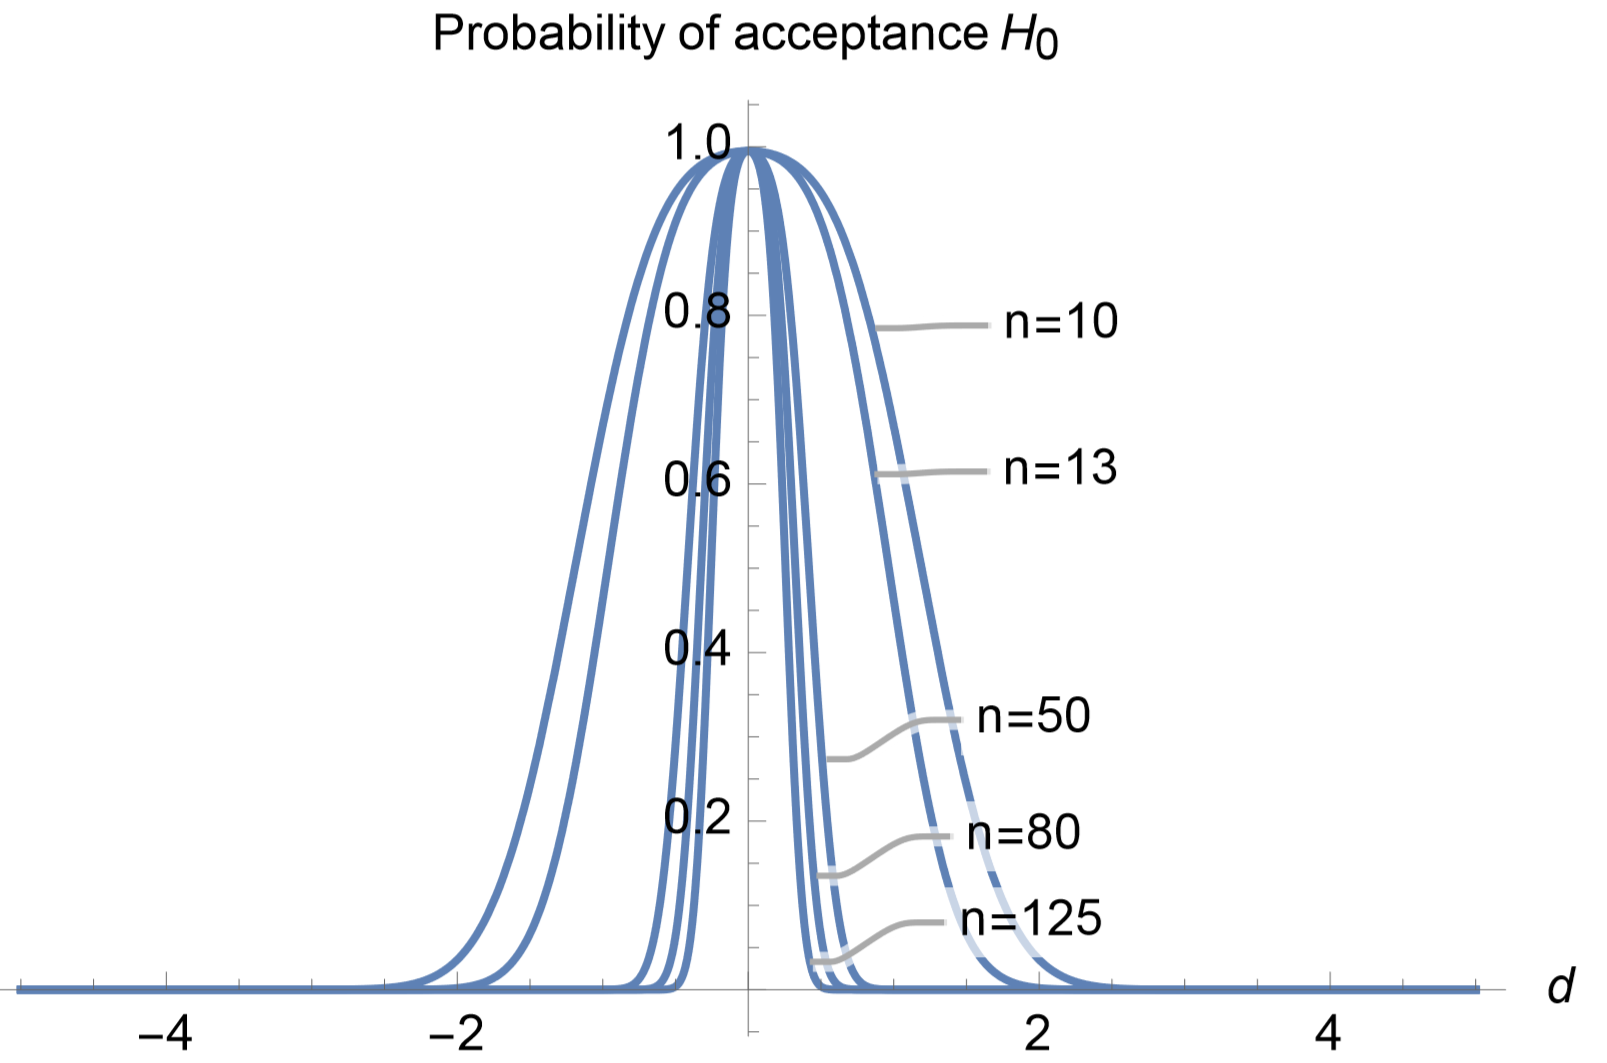
\includegraphics[width=0.8\linewidth]{occurve1.png}  
\caption{The OC Curves of the Test in Table 4} 
\label{fig1}
\end{figure}

\newpage

We alternatively give the plots for other null hypothesis for comparison.

\begin{figure}[!htbp] 
\centering 
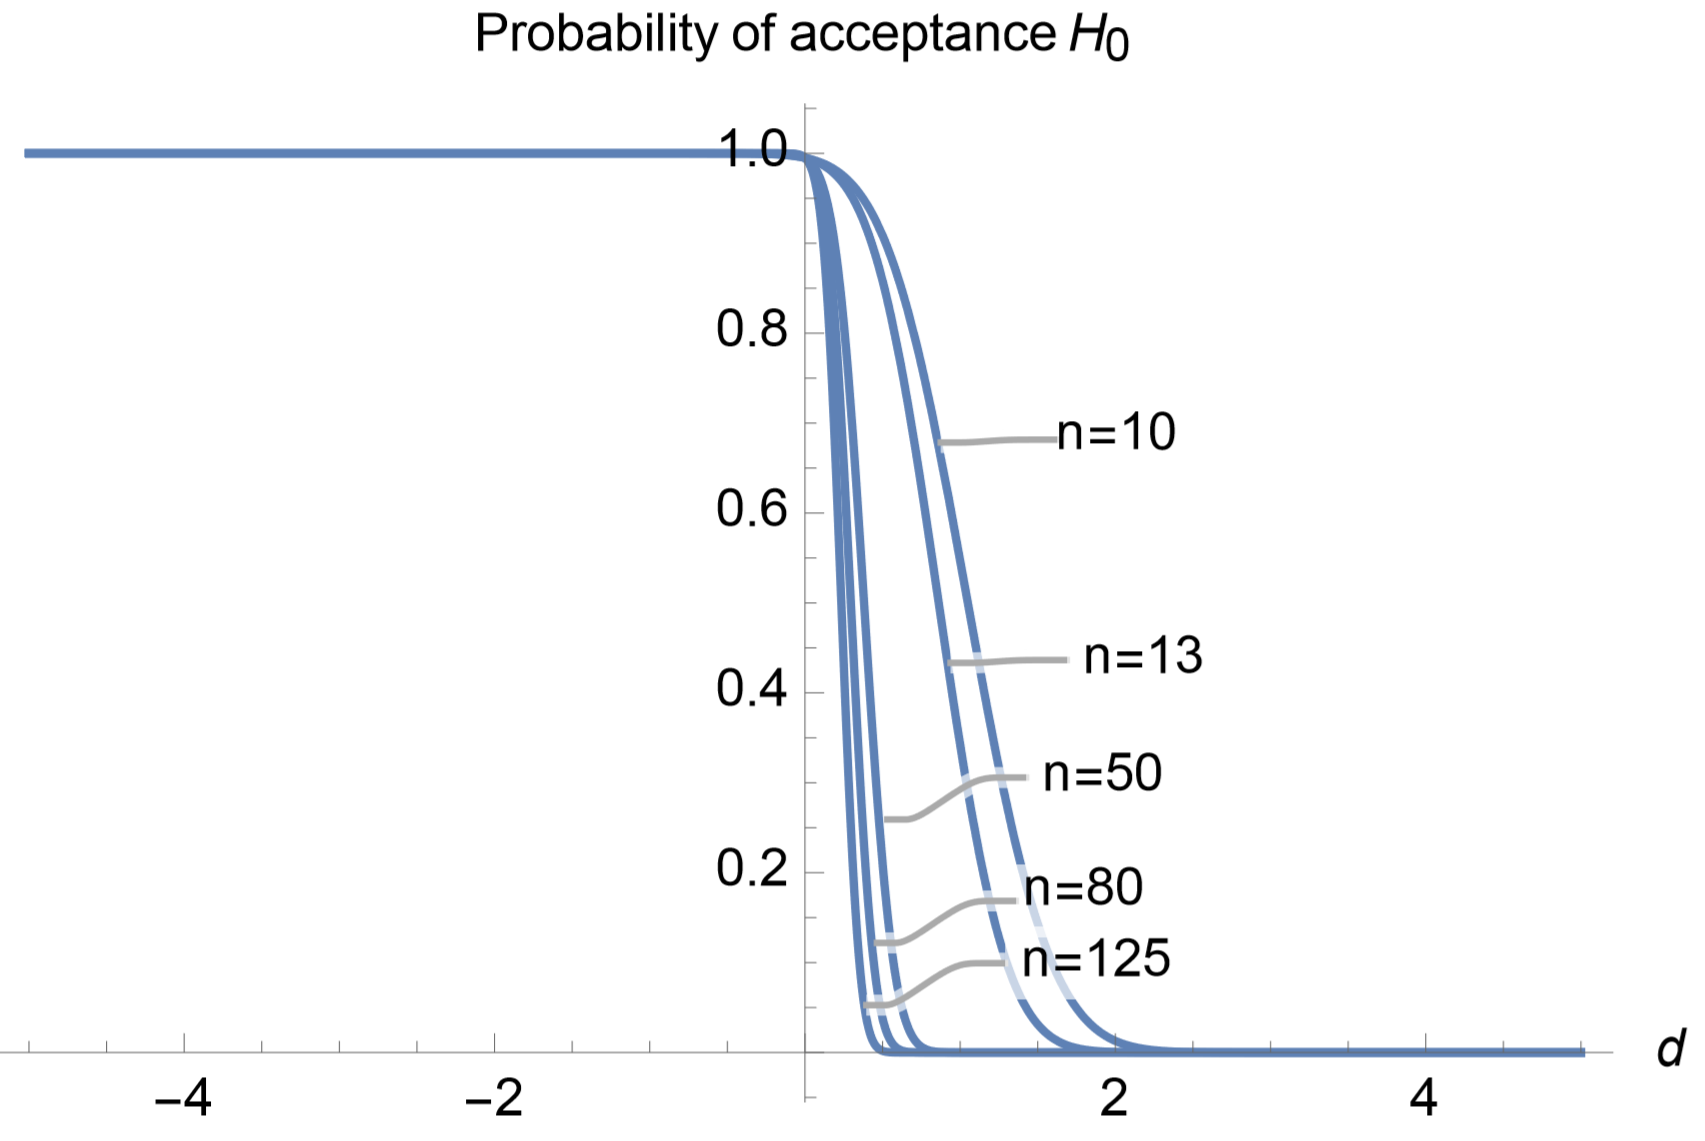
\includegraphics[width=0.8\linewidth]{occurve2.png}  
\caption{The OC Curves of the Test in Table 4, $H_0: \mu\leq Q_n$} 
\label{fig1}
\end{figure}

\begin{figure}[!htbp] 
\centering 
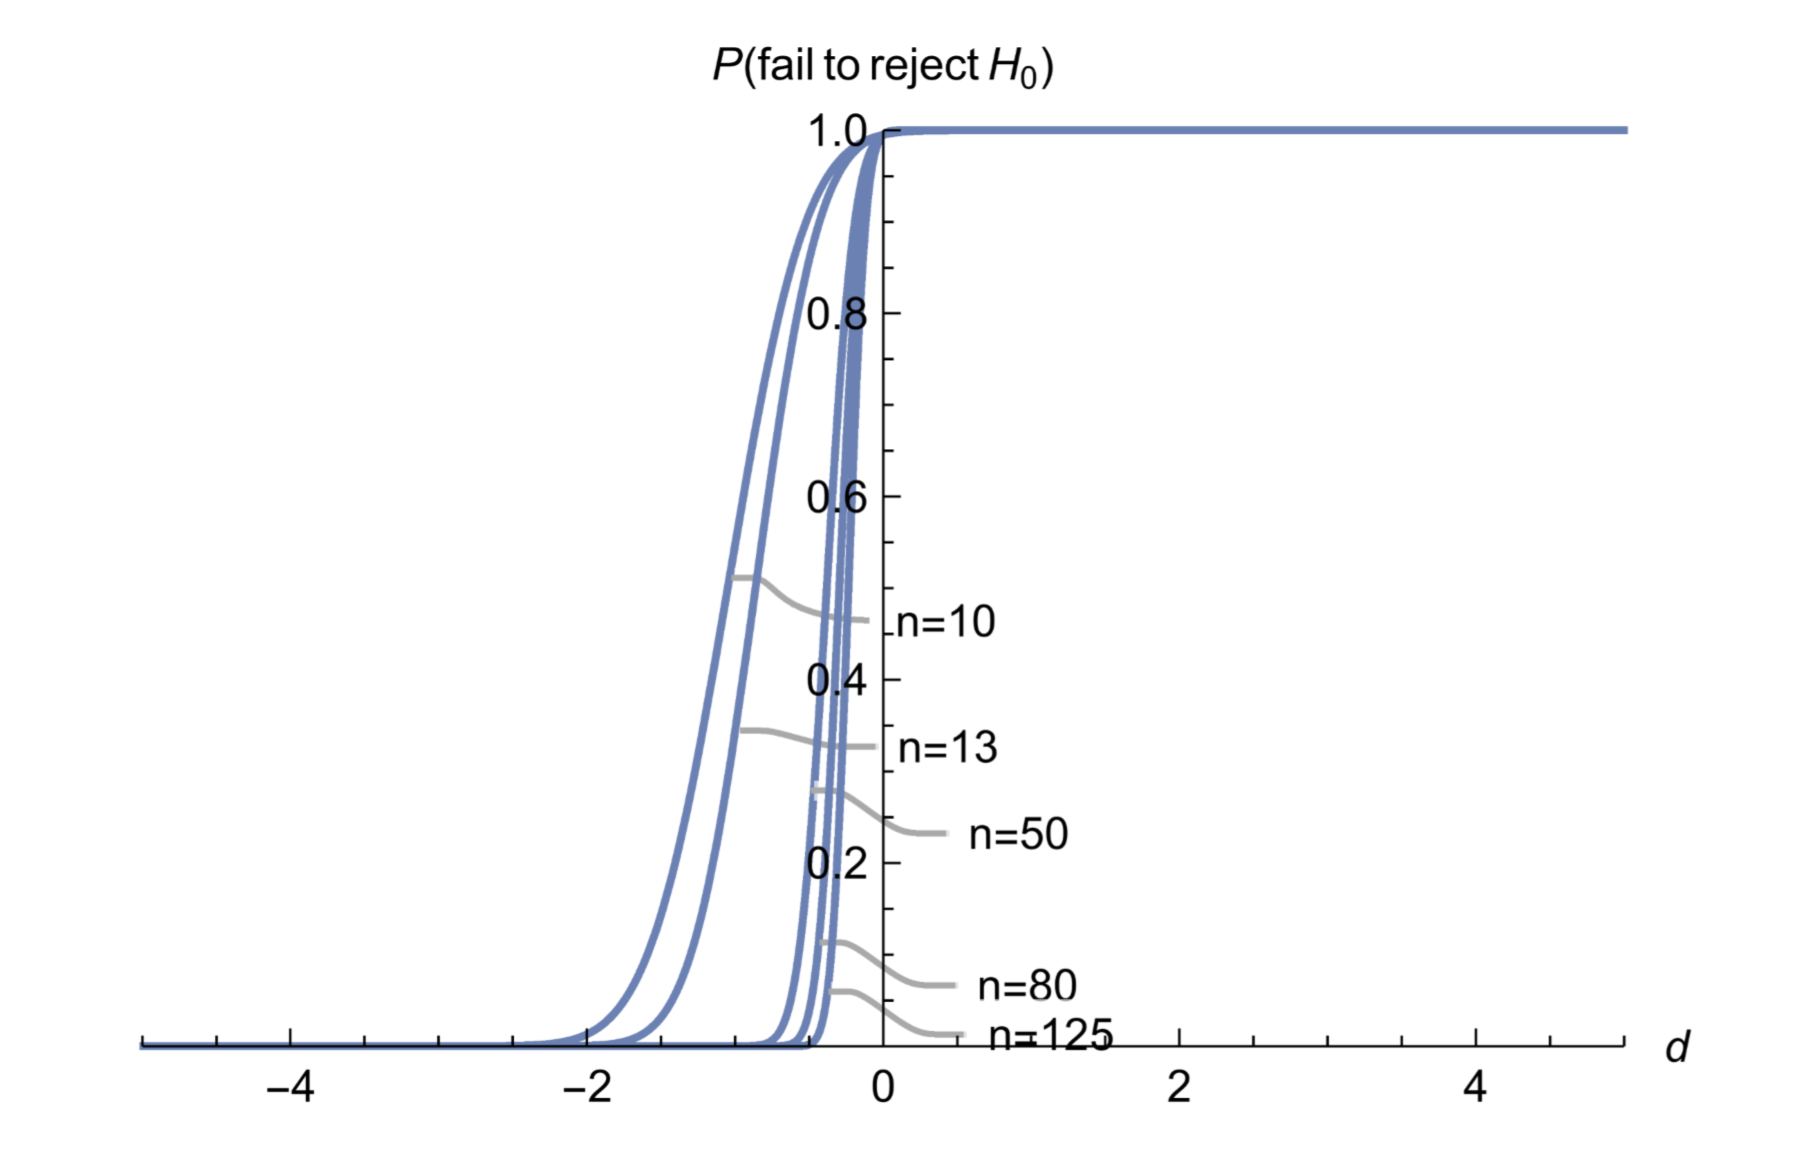
\includegraphics[width=0.8\linewidth]{occurve3.png}  
\caption{The OC Curves of the Test in Table 4, $H_0: \mu\geq Q_n$} 
\label{fig1}
\end{figure}

\newpage

\subsection{Power of the Tests}
Power is defined as $1-\beta$. Since $\beta$ defines the probability that we accept $H_0$ even though $H_1$ is true, the meaning of power is that it defines the probability of successfully rejecting a false $H_0$ given that $H_1$ is true.

$$\text{power} = P[\text{reject }H_0\ |\ H_1 \text{ is true}]$$

We noticed that The OC Curve is a plot of $1 - P[\text{reject }H_0]$ against some parameter that can be determined if $H_1$ is true, i.e. if $H_1$ is true, we can find the value of $d$ and read the power from the $y-$axis. \textbf{Hence, $\beta$ corresponds to a point on OC curve, and power is $1-\beta$.}

Observations show that:
\begin{itemize}
    \item Let d and $\alpha$ be unchanged. When $n$ increases, $\beta$ decreases and power increases.
    \item Let $\alpha$ and n be unchanged. We will get $|\mu-\mu_0|$ from data and thus d. Then we will get a point on the vertical coordinates. 
\end{itemize}

This identifies with the equation $\displaystyle n \approx \frac{(z_{\alpha/2}+z_\beta)^2\sigma^2}{\delta^2}$ in [3], where we can see that when $n$ increases, $\beta$ decreases and power increases. As long as n is large enough, one can always reject $H_0$, which decreases the customer's risk.

\newpage

\subsection{Probability of Detecting a Shortfall of at Least One Standard Deviation}
\begin{itemize}
    \item When $N$ $\geq$ 11, we get a sample from products, where $n$ is the size of sample. The probability is that we detect a sample mean $\overline{q}$ with a shortfall of at least one sample standard deviation $s$ from the nominal net quantity $Q_n$.
    \begin{align*}
        P[\overline{Q} \leq Q_n - s]
        &=P[\frac{\overline{Q} - Q_n}{s/\sqrt{n}}\leq \frac{Q_n - s - Q_n}{s/\sqrt{n}}]\\
        &=P[\frac{\overline{Q} - Q_n}{s/\sqrt{n}}\leq-\sqrt{n}]\\
    \end{align*}
    
    As is discussed, $\displaystyle\frac{\overline{Q} - Q_n}{s/\sqrt{n}}$ follows Non-central T Distribution.
    \begin{align*}
        P[\overline{Q} \leq Q_n - s]
        &=P[T_{n-1} \leq -\sqrt{n}]\\
        &=F_{n-1,d\sqrt{n}}(-\sqrt{n})
    \end{align*}
    
    When $d=0$, $H_0$ is assumed true. This is equal to ask, in $\overline{q}\leq Q_n-\lambda s$ when the modifying factor $\lambda=1$, find the corresponding confidence level of each $n$.
    \item When $N$ $\leq$ 10, we test all the items. Hence $\sigma$ and mean $\mu$ of the products are known.
    
    When N $\leq$ 10, $n=N$ is the size of batch. The probability is that we detect a mean $\overline{q}$ with a shortfall of at least one standard deviation $\sigma$ from the nominal net quantity $Q_n$.
    
    \begin{align*}
        P[\overline{Q}\leq Q_n -\sigma]
        &=P[\frac{\overline{Q}-\mu}{\sigma/\sqrt{N}}\leq \frac{Q_n -\sigma-\mu}{\sigma/\sqrt{N}}]
    \end{align*}
    
    $\displaystyle\frac{\overline{Q}-\mu}{\sigma/\sqrt{N}}$ follows Standard Normal Distribution.
    \begin{align*}
        P[\overline{Q}\leq Q_n -\sigma]
        &=P[Z\leq \frac{Q_n -\sigma-\mu}{\sigma/\sqrt{N}}]\\
        &=\Phi [\frac{Q_n -\sigma-\mu}{\sigma/\sqrt{N}}]
    \end{align*}
\end{itemize}

\newpage

\section{Significance Level of Type I Error}
\subsection{Summary of Section 5.3.2 in [1]}
\paragraph{Significance of T-Test}
Section 5.3.2.1 corresponds to the T-Test for sample mean net quantity. To summarize, for inspection lot satisfying $\mu=Q_n$, the probability of being rejected is not more than $0.5\%$.

To make it understandable for manufacturers, the quality supervision departments display formula $\overline{q} \geq (Q_n-\lambda s)$ where $\lambda$ is shown in the third column in Table 4. The meaning is that the average sample content should be not less than the label net content minus the product of correction factor $\lambda$ and the standard deviation of the sample. 
\paragraph{Significance of Acceptance Sampling}
Section 5.3.2.1 corresponds to the acceptance sampling for detective rate. To summarize, for inspection lot satisfying the fact that the percentage of shortage quantitative packaged goods is not more than $2.5\%$, the probability of being rejected is not more than $5\%$.

To be more specific, the shortage quantitative packaged goods include both $ T_{1} $ shortfall products and $ T_{2} $ shortfall products. It can be used to calculate the allowed amounts of  $ T_{1} $ shortfall and $ T_{2} $ shortfall, which is shown in the forth column in Table 4 in JTF 1070-2005.

\subsection{Discussions of the Statements}
From above discussions, the significant value $ \alpha $ can be approximately calculated as:
\begin{equation}
    \alpha \approx \sum_{d>c} \frac{(n\Pi_0)^d e^{(-n\Pi_0)}}{d!}
\end{equation}
in which $\Pi_0=2.5\%$ and c is shown in Table 4 as 0,0,1,3,5,7. d is min (n,r) where $r=floor(N\Pi_0)$.

Both significant levels above are usually called the Type I error($ \alpha $) or the producer's risk. On one hand, it guarantees the profit of producers by limiting the probability of rejection. On the other hand, it shows the maximum allowed Type $ T_{1} $ and  $ T_{2} $ shortfall. The specific calculation is displayed in the above analysis. In the Section 4.3.1, we discuss the level of Type I error using three methods including hypergeometeric distribution, approximating binomial and poisson distribution. Table 3 and 4 show the corresponding $ \alpha $ value which is quite larger than the threshold value 5\% when the sample amount is small. The tables also show a tendency of $ \alpha $ to decrease below 5\%. Some reasons can explain this abnormal Type I error:
\begin{itemize}
\item The 0.5\% siginificant value limits the mean of the products and the 5\% significant value limits the passing rate. The abnormal value in Table 3 and 4 can be caused by the balance of producer's risk and consumer's risk. 
\item Noticing when the inspection lot amount is larger than 3200, the sample amount is 125. In Table 3 and 4, the corresponding $ \alpha $ value is below 5\%. In manufacturing, the larger amount of the products in prepackages with fixed content, the more necessary to control its cost. Rejecting too many acceptable products not only wastes materials but also increases the cost. Such as the car wheels production, the small preset $ \alpha $ value protects the manufacturer's profit. Similarly, when the inspection lot has a rather small amount, the high level of rejection probability ensures the quality of the products. Owing to the small amount, the manufacturer can improve the process better. 

\item Consideration that $T_2$ shortfall will be taken into account for smaller $Q_n$. Note that in the previous sections, we have assume that $T_2$ shortfalls are ignorable.

\begin{figure}[!htbp] 
\centering 
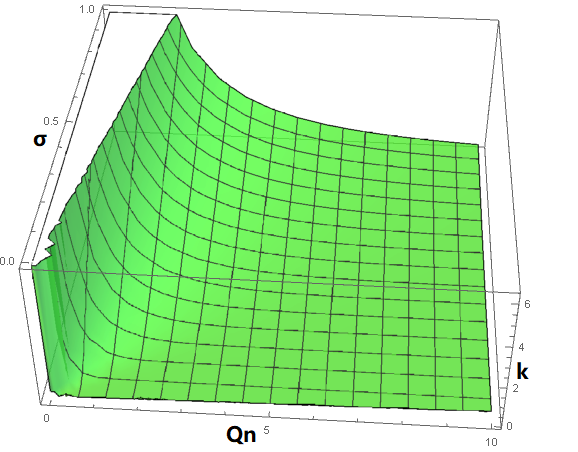
\includegraphics[width=0.6\linewidth]{T12.png}  
\caption{The Plot of $k$ against $\sigma$ and $Q_n$} 
\label{fig1}
\end{figure}

However, for batch of products with small $Q_n$ and large $\sigma$, this is not the case. For example, we fix $\sigma=1$ and $\mu=Q_n=5$, we can calculate the $k$ value is only:
$$k = 1.29351$$

This would mean that a $T_2$ shortfall will be detected more possibly than a $T_1$ shortfall!

\item Consideration of a barely acceptable $\Pi_1$.

We assume that for larger $N$, we define $H_1: \Pi > \Pi_1 = 0.12$, and plot the $c$ versus $N$ using Hypergeometric distribution. The result is as follows.

\begin{figure}[!htbp] 
\centering 
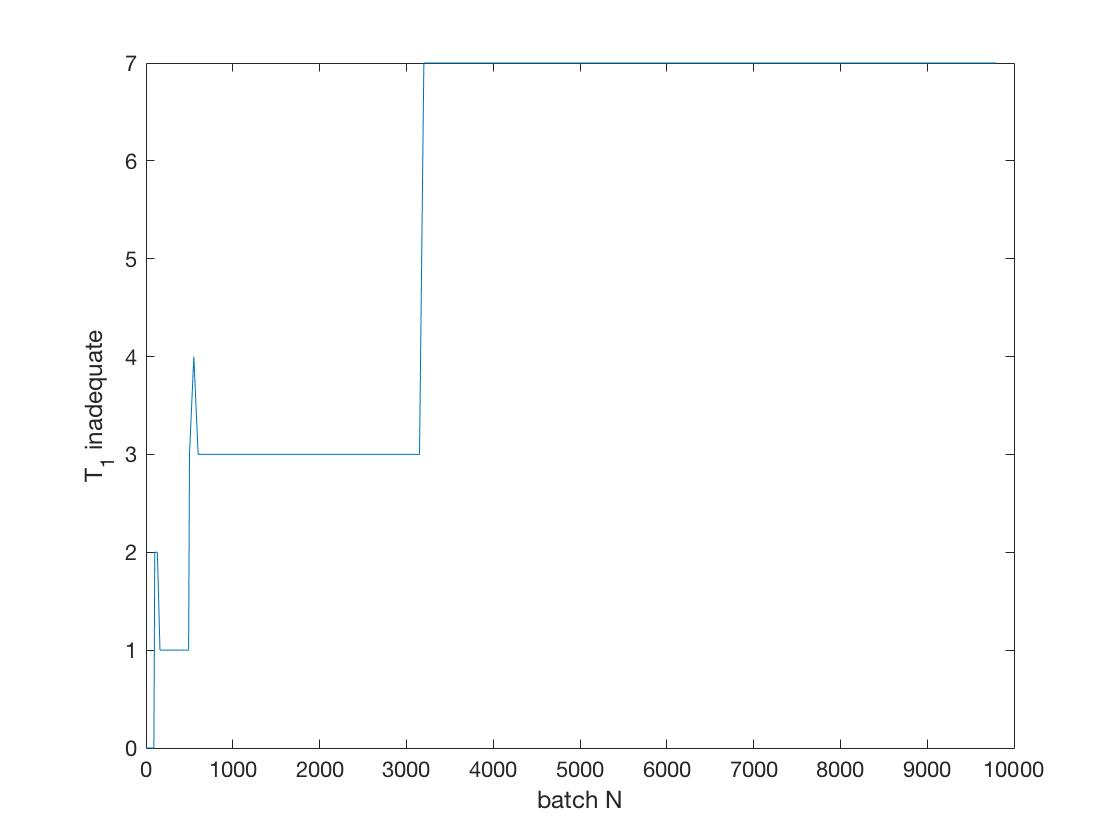
\includegraphics[width=0.7\linewidth]{beta-hyper-pi1.jpg}  
\caption{The Relationship between $c_{\max}$ and $N$, Hypergeometeric, $\Pi_1=0.12$} 
\end{figure}

We found that for larger $N$, $c=7$ is true.
\end{itemize}


\newpage

\section{Tests of a Sample of Prepackaged Food}
\subsection{Objectives}
The goal of this exercise is to test on a package of DOUBLEMINT pressed candies and verify whether the actual package contents correspond to the nominal contents according to JTF 1070-2005.

\subsection{Testing Materials and Apparatus}
DOUBLEMINT pressed candies, electronic weigh.
\subsubsection{Testing Materials}
\begin{figure}[!htbp]
\centering

\includegraphics[width=0.5
\linewidth,angle=0]{sample.jpg}
\caption{DOUBLEMINT pressed candies}
\end{figure}

\begin{table}[!htbp]
\centering
\begin{tabular}{|c|c|}
\hline
Net weight&12g
\\\hline
Production date&2018.08.15
\\\hline
Shelf life&12 months
\\\hline
\end{tabular}
\caption{Main Labels on the Package}
\end{table}

\subsubsection{Apparatus}
Electronic scales
\begin{figure}[!htbp]
\centering

\includegraphics[width=0.5
\linewidth,angle=0]{scale.jpg}
\caption{Electronic Scale}
\end{figure}


\begin{table}[!htbp]
\centering
\begin{tabular}{|c|c|}
\hline
Units&g
\\\hline
Accuracy&0.1g
\\\hline
Capacity&1000g
\\\hline
Operation Temp&10 to 30 dec C
\\\hline
\end{tabular}  
\caption{Main Parameters of the Scale}
\end{table}

\subsection{Procedure}
\subsubsection{Measurement of average tare weight}
\begin{itemize}
\item Select two packages from the sample. Measure the difference of their net weight ($R_c$) and the difference of the tares ($R_t$).
\item Choose the number of packages in the sample that we need to measure the tares($n_i$) with the value $R_c / R_t$ according to Table B.2.
\item If $R_c / R_t$ $\leq$ 1.00, test the weight of every tare as the tare weight of the package. Else we test the average weight of all $n_i$ tares as  the tare weight.
\end{itemize}

\begin{figure}[!htbp]
\centering

\includegraphics[width=0.4
\linewidth,angle=0]{net.jpg}
\caption{Measurement of Net Weight}

\includegraphics[width=0.4
\linewidth,angle=0]{tare.jpg}
\caption{Measurement of Tare Weight}

\includegraphics[width=0.4
\linewidth,angle=0]{general.jpg}
\caption{The general weight of package}
\end{figure}

\subsubsection{Measurement of the actual content deviation}
\begin{itemize}
\item Measure the general weight ($GW_i$) of every package.
\item Calculate the actual content ($q_i$) of every package with the equation $q_i = GW_i - \overline{P}$.
\item Calculate the content deviation of every package ($D_i$) with the equation $D_i = q_i - Q_n$.
\end{itemize}

\subsection{Measurements and Results}
We had 99 packages of DOUBLEMINT pressed candies which was the inspection lot. According to [3, Table 4],  we chose 13 of them as the sample that we tested on. For convenience, we labelled them from Package 1 to 13.
\subsubsection{Measurement of average tare weight}
Select Package 1 and 2 and we measured:
\begin{table}[!htbp]
\centering
\begin{tabular}{|c|c|c|}
\hline
i&Net weight(measured)\ [g]&Tare weight(measured)\ [g]
\\\hline
1&12.8&8.4
\\\hline
2&12.8&8.3
\\\hline
\end{tabular}  
\caption{Net and Tare Weight of the Samples}
\end{table}

Since the measured $R_c=0$, we chose `$R_c/R_t \leq 0.2$' in Table 2. The corresponding tare sample number $n_i$ is 13. $n_i = n$, so we would need to measure the actual tare weight for every package.
\begin{table}[!htbp]
\centering
\begin{tabular}{|c|c|c|c|c|c|c|c|c|}
\hline
i&Tare weight(measured)\ [g]&i&Tare weight(measured)\ [g]&i&Tare weight(measured)\ [g]
\\\hline
1&8.4&2&8.3&3&8.3
\\\hline
4&8.3&5&8.0&6&8.3
\\\hline
7&8.3&8&8.3&9&8.4
\\\hline
10&8.6&11&8.4&12&8.3
\\\hline
13&8.4&&&&
\\\hline
\end{tabular}  
\caption{All Measurements of Tare Weights}
\end{table}

\subsubsection{Actual content deviation}
The results are as follows.

\begin{table}[!htbp]
\centering
\begin{tabular}{|c|c|c|c|c|}
\hline
i&$GW_i\ [g]$&$q_i=GW_i-\overline{P}\ [g]$&$Q_n\ [g]$&$D=q_i-Q\ [g]$
\\\hline
1&21.2&12.8&12&0.8
\\\hline
2&21.1&12.8&12&0.8
\\\hline
3&21.1&12.8&12&0.8
\\\hline
4&21.1&12.8&12&0.8
\\\hline
5&21.2&13.2&12&1.2
\\\hline
6&20.9&12.6&12&0.6
\\\hline
7&21.1&12.8&12&0.8
\\\hline
8&21.2&12.9&12&0.9
\\\hline
9&21.2&12.8&12&0.8
\\\hline
10&21.4&12.8&12&0.8
\\\hline
11&21.2&12.8&12&0.8
\\\hline
12&21.4&13.1&12&1.1
\\\hline
13&21.2&12.8&12&0.8
\\\hline
\end{tabular}
\caption{Calculation of Actual Content Deviation} 
\end{table}

\newpage

We can then plot the boxplot of the obtained data.
\begin{figure}[!htbp]
\centering
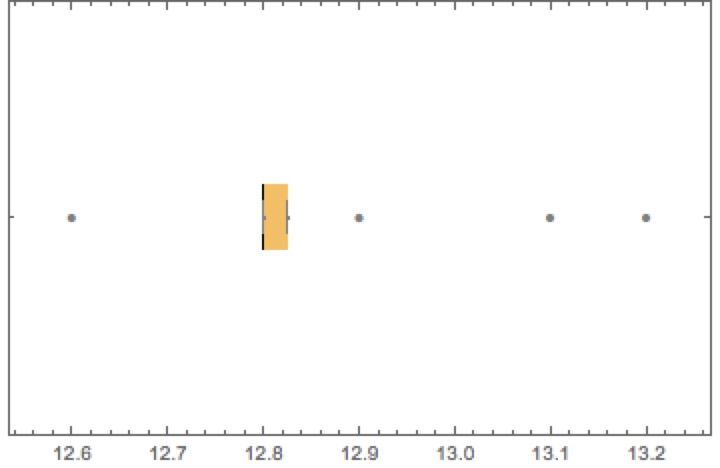
\includegraphics[width=0.8
\linewidth,angle=0]{Boxplot.jpg}
\caption{The boxplot of sample weight}
\end{figure}

\subsection{Analysis}
First we calculate the average content of samples:
\begin{align*}
\overline{q}&=\frac{1}{n}\displaystyle\sum^n_{i=1}q_i
\\&=\frac{1}{13}(12.8*9+13.2+13.1+12.6+12.9) [g]
\\&=12.85 [g]
\end{align*}

Then we get the standard deviation of the sample actual contents:
\begin{align*}
s&=\sqrt{\frac{1}{n-1}\displaystyle\sum^n_{i=1}(q_i-\overline{q})^2}
\\&=\sqrt{\frac{1}{12}(0.05^2\times 10+0.25^2\times2+0.35^2)} [g]
\\&=\sqrt{\frac{1}{12}\times0.2725} [g]
\\&=0.151 [g]
\end{align*}

In Table 4, the modifying factor $\lambda = t_0.995*\frac{1}{\sqrt{n}}$ = 0.848 when n = 13 is provided, so we have:
\begin{equation*}
Q_n-\lambda s = 12-0.848\times0.151\ [g]= 11.87\ [g]
\end{equation*}
\par Thus, we have clear evidence applying the testing rules for net quantities of a batch:
\begin{itemize}
\item The average content of samples $ \overline{q}=12.85\ [g] $ is larger than the net quantity minus the actual average quantity modification value $ Q_{n} - \lambda  s = 11.87\ [g]$.\
\item The number of type $T_{1}$ shortfalls is less than the preset acceptance number 1. 
\item No type $T_{2}$ shortfalls occurs for the sample weights are all larger than the net quantity. 
\end{itemize}
\par In all, the package of DOUBLEMENT pressed candies \textbf{accords with} the measurement requirements in JTF 1070-2005. 
\par Further, something needs to be noticed: 
\begin{itemize}
\item The standard deviation s has a rather small value 0.151g. In Figure 13, we can see four points are near outliers and the distance between adjacent values is rather small. Thus, there is evidence of this small deviation and symmetrical feature. The larger standard deviation s is, the more necessary to increase the preset mean of normal distribution in manufacturing to reduce the consumer's risk. This undoubtedly increases the average cost of production. So a wiser way is to improve the accuracy of the production machine. 
\item Our sample weights are all larger than the nominal quantity.  The 99.5\% confidence interval ensures most of the sample net quantity is much larger than the nominal quantity. 
\item The amount of inadequate products in prepackages with fixed content is strictly limited. When the shortfall occurs (especially type $T_{1}$ shortfall), finding the reason for the abnormal fluctuation is on the top priority. After eliminating the interfering factor, we can do the sampling inspection again and put back on production.  If the type $ T_{2} $ shortfall is detected, it means the production machine has a lower accuracy of manufacturing. Then the production should be stopped immediately and manufacturer should rectify and reform the process capability.  
\item The confidence coefficient is 99.5\% rather than 100\% in this metrology inspection. There exists the Type II error($ \beta $) during the inspection. Generally, we use other methods to lower this risk such as `Six Sigma' strategies [5], control chart [6] and process capability index etc. 
\end{itemize}

\section{Conclusion}
In conclusion, the project investigate the \textit{Rules of metrological testing for net quantities of products in prepackages with fixed content}, issued by Chinese government in 2005.

Specifically, we are interested in the mean testing and acceptance sampling methods and rules that Chinese government predetermined to measure the net quantity of a batch of products and control the type I error (rejecting an acceptable lot) and type II error (failing to reject an unacceptable lot) by verification of the significance and acceptance numbers.

We successfully conduct tests with accord to the document, in order to verify whether or not the actual quantity of DOUBLEMINT sample corresponds to its labelled contents. We finally conclude that the package of DOUBLEMENT pressed candies \textbf{accords with} the measurement requirements in JTF 1070-2005. 

\newpage

\section{References}
\subsection{Works Cited}
%[1] 全国法制计量管理计量技术委员会/定量包装商品净含量工作组. 定量包装商品净含量计量检测规则 (Rules of metrological testing for net quantities of products in prepackages with fixed content). \textit{Technical Report JJF 1070-2005}, 中国计量出版社(China Metrology Publishing House), 2005. \url{http://www.ahhz.gov.cn/CountyOpennessContent/show/ 1078758.html} [Online; accessed 22-March-2019].

[1] Rules of metrological testing for net quantities of products in prepackages with fixed content. \textit{Technical Report JJF 1070-2005}, China Metrology Publishing House, 2005. \url{http://www.ahhz.gov.cn/CountyOpennessContent/show/ 1078758.html} [Online; accessed 22-March-2019].

[2] Requiem for the Truth-in-Packaging Bill? \textit{Journal of Marketing}, Vol.30, No.2 (Apr 1966), pp. 1-5, JSTOR. \url{https://www.jstor.org/stable/1249054} [Online; accessed 3-April-2019].

[3] H. Hohberger. "ve401\uline{ }main.pdf"(2018). UMJI-SJTU, Shanghai. [Online; accessed 25-Feb-2019]. 

[4] Wikipedia. Noncentral t-distribution, \textit{wikipedia}, the free encyclopedia, 2014. \url{https://en.wikipedia. org/wiki/Noncentral_t-distribution} [Online; accessed 10-April-2014]. 

[5] Wikipedia. Six Sigma, \textit{wikipedia}, the free encyclopedia, 2014. \url{https://en.wikipedia. org/wiki/Six_Sigma} [Online; accessed 10-April-2014]. 

[6] Wikipedia. Control chart, \textit{wikipedia}, the free encyclopedia, 2014. \url{https://en.wikipedia. org/wiki/Control_chart} [Online; accessed 10-April-2014]. 
\subsection{Figures}
[I] \url{https://en.wikipedia.org/wiki/Central_limit_theorem#/media/File:Central_Limit_Theorem.png}

\section{Appendix}
\subsection{\texttt{Mathematica} and \texttt{Matlab} Codes}
\end{document}
